\documentclass{vldb}

%\setcopyright{rightsretained}



\usepackage{booktabs}
\usepackage{graphicx}
\usepackage{balance}  % for  \balance command ON LAST PAGE  (only there!)
\usepackage[caption=false,font=footnotesize]{subfig}
\usepackage{amsmath}
\usepackage{amsopn}
\usepackage{comment}
\usepackage[ruled,linesnumbered]{algorithm2e}
\usepackage{multirow}
\usepackage{enumitem}
\usepackage{color}
\usepackage{listings}% http://ctan.org/pkg/listings
\lstset{
  basicstyle=\ttfamily,
  mathescape
}
\newcommand{\tabincell}[2]{\begin{tabular}{@{}#1@{}}#2\end{tabular}}

\hyphenpenalty=5000
\tolerance=500

\begin{document}

%
% paper title
% can use linebreaks \\ within to get better formatting as desired
\title{A3Log: Automated Asynchronous Evaluation for Recursive Datalog Programs}

% author names and affiliations
% use a multiple column layout for up to three different
% affiliations

% conference papers do not typically use \thanks and this command
% is locked out in conference mode. If really needed, such as for
% the acknowledgment of grants, issue a \IEEEoverridecommandlockouts
% after \documentclass

% for over three affiliations, or if they all won't fit within the width
% of the page, use this alternative format:
%
\author{}

% make the title area
\maketitle


\begin{abstract}


%Synchronous aggregation in parallel and distributed computing is the root reason of low efficiency. On the other hand, asynchronous aggregation is promising, which breaks up synchronization barriers and allows coordination-free execution. However, asynchronous aggregation suffers from the problems of non-guaranteed correctness and non-deterministic performance due to the possible redundant computations and communications. Moreover, asynchronous program is a lot harder to write, tune, and debug. To address these issues, we propose A3, Automatic Asynchronous Aggregation. Based on A3, we design and implement a Datalog system, A3Log, which provides both shared-memory runtime engine and distributed runtime engine. Our results on Amazon EC2 show that asynchronous execution can achieve up to two-orders-of-magnitude speedup over synchronous counterpart.
\end{abstract}
%%With A$^3$ theory, asynchronous aggregation of recursive program is guaranteed to return correct result and achieve better performance, and a recursive program can be automatically converted for asynchronization.

\keywords{Asynchronous aggregation, parallel aggregation, recursive program, Datalog}



\newcommand{\Paragraph}[1]{\smallskip\noindent{\bf #1.}}
\newtheorem{theorem}{\textbf{Theorem}}
\newtheorem{lemma}{\textbf{Lemma}}
\newdef{definition}{\textbf{Definition}}


\section{Introduction}
\label{sec:intro}

With the increasing of sensor performance and the rapid expansion of social network data, it is necessary to parallelize or distribute the analysis and computation of large scale data. However, the parallelization of algorithms requires programmers to have a rich knowledge of distributed systems. A large number of big data analysis systems have been proposed which provide high-level language for expressing the computation logic \cite{}. Even so, these systems still require the users to understand the specific programming logic. For example, the typical representative of the BSP computing model, Pregel \cite{} adopts a vertex-centric programming model. It requires programmers to write vertex-centric programs and to manage the communication based on the algorithm. 

%Maiter[$]is an asynchronous graph computing system which proposed a delta-based accumulative iterative computation method. Maiter provide an asynchronous programming model, demand the programmer rewrite the algorithm in a DAIC way. The complexity of parallize or distribute an algorithm wasn��t significantly reduced.


%Its core advantage to  relational query languages is its elegant notation for expressing recursion.but it is not widely adopted as practical query language because of the lack of negation. In particular, it cannot express even the first-order queries which limited the usage.While since 2010 datalog is getting  more popular due to the graph/social network processing requirement. 

New interest has recently re-emerged around Datalog for a wide spectrum of knowledge-oriented applications \cite{Bigdatalog 25,27,64,47,49}.
%[25], AI [27], and distributed data management [64], as well as analytics on single-node systems [47, 49]. The fact that Datalog is also well suited to declaratively support large-scale analytics was recently recognized by [48, 54].
Datalog is an excellent candidate language for large-scale data analytics because of its high-level declarative semantics and support for recursion. Datalog's support for recursion makes the expression of data analysis natural \cite{} and its high-level semantics makes it amenable to parallelization and optimization \cite{}. 
%Although many advantages it has��the performance of Datalog is not competitive when compared with other languages.
In recent years, many system research efforts have raised to improve the performance and scalability of Datalog systems. Socialite \cite{socialite} provides a large scale graph evaluation system supporting both sequential and distribute environment. In Socialite, users can define recursive aggregate functions which, as long as they are meet operations, can be evaluated incrementally and efficiently. The \textit{DeALS} project provides a full Datalog language implementation and seeks to provide  system supports that optimizes execution over diverse platforms including sequential implementations \cite{bigdatalog 49}, multi-core machines [59], and clusters \cite{bigdatalog}. It supports relational algebra, aggregation, and recursion, as well as a host of declarative optimizations. MyriaX \cite{} implements a Datalog System on share-nothing engines based on Myria \cite{}. The computations are incremental, and it support s a variety of iterative models (synchronous, asynchronous, different processing priorities) and failure-handling techniques. It is worth mentioning that MyriaX supports asynchronous processing and shows promising performance for some applications, but it fails to tell in which cases asynchronous processing is suited.

%It is worth mentioning that MyriaX is the first work that proposed recursive program with aggregation.And  inspired by this work.We present arbitary recurive parallel algorithm with two type of operations  aggregattion and non-aggregation in our approach which makes it more convenient to analyze and parallize.We will discuss in detail later in this paper. 
%[$Myria],a big data management system.[���������ص�ǿ���첽] It is worth mentioning that MyriaX is the first work thatUsually support recursive program with aggregation.


Compared with synchronous recursive processing, asynchronous recursive processing has many advantages, such as fast convergence \cite{}, more efficient resource utilization \cite{}, and priority scheduling \cite{}. However, in practical usage, synchronous systems are more popular than asynchronous systems, which can be attributed to the following three points:

First, \textbf{Non-guaranteed Correctness}. There are several prior works that have employed asynchronous processing engine for improving their system performance. However, these systems only implement asynchronous execution of parallel/distributed algorithms, without any correctness guarantee of the results \cite{groute, graphlab,...}. Asynchronous computation model are blindly used and may result in inconsistent results for convex functions. Maiter \cite{} provides the sufficient conditions for correct asynchronous computations, but these conditions are only suitable in the context of vertex-centric graph computations. 

Second, \textbf{More Complexity}. Programmers are used to write sequential programs or synchronous parallel programs. Had the asynchronization conditions been formally given, it is still hard for a non-expert programmer to manually verify these conditions from their programs. In addition, writing asynchronous programs and designing asynchronous systems are even harder, because asynchronous implies disorganized and as a result complicated. Experience from Google \cite{} strongly suggests a synchronous programming model, since asynchronous code is a lot harder to write, tune, and debug. 

Third, \textbf{Unstable Performance}. Asynchronous iterative processing avoids the intermediate result coordination phase. The parallel executions of operations are not synchronized and not strictly ordered. This implies that the computations and communications are not under control any more, which may lead to stale computations/communications and potentially reduces the efficiency. The performance gain from asynchronous computation may be not enough to compensate for the performance loss from stale computations/commmunications, leading to unstable performance.


In order to solve these problems, we design and implement a Datalog system supporting automated asynchronous execution, A3Log. Our system is able to automatically check whether a recursive Datalog program can return correct result with asynchronous recursive execution. This is achieved by automated sufficient conditions verification. Maiter \cite{} provides the sufficient conditions for asynchronous graph processing. In this paper, we generalize the sufficient conditions through the analysis of aggregate and non-aggregate operators, which can be easily identified from a user's Datalog program. Aggregate operation is known to be hardly parallelized \cite{distribute aggregate from ms}, while non-aggregate operation can be embarrassingly parallel. Synchronization of parallel computations seems to be the unavoidable coordination step for correct aggregation result though it is known costly. Our new sufficient conditions are provided by analyzing the properties of aggregate operations and non-aggregate operations. A3Log can also automate the condition verification process without user's participation. Further, A3Log provides both shared-memory runtime engine and distributed runtime engine for fast execution. 


%For example, MapReduce \cite{} decomposes a computation into (non-aggregate) map operations and (aggregate) reduce operations so as to parallelize the non-aggregate map operations and parallelize the reduce operations separately. But the synchronization barrier before reduce phase is indispensable due to the aggregation property. Given the aggregate operation and non-aggregate operation learned from user's Datalog program, A3Log is able to

%correctly asynchronized according to a novel Sufficient Condition by datalog program.Note that,different from the previous work Maiter[] which proposed asynchronous condition of graph algorithm .Our approach is based on aggregation operation and more generalized to apply on more algorithm except graph analysis .Such that Asynchronous calculations needn��t to be used blindly. And the workload of the programmer is greatly reduced. In order to meet different use requirements, system provides both  shared-memory runtime engine and distributed runtime engine. The contribution are summarized as follow

The contributions of this paper are summarized as follows.
\begin{itemize}
\item To guarantee the correctness of recursive Datalog program, we clearly define the sufficient conditions that guarantee asynchronous processing to return the same result as synchronous processing through the analysis of aggregate and non-aggregate operators. Even for some recursive programs that do not satisfy these conditions, we propose an approach to conditionally convert them to be qualified for asynchronous aggregation. 
\item To alleviate the burden of programmers, we propose an automated condition verification technique by leveraging satisfiability modulo theories
(SMT) . User?s sequential program can be automatically checked for asynchronization possibilities and can even be automatically converted to the asynchronous program.
\item We propose a Datalog implementation, A3Log, to support automated asynchronous aggregation. A3Log is built by modifying distributed Socialite \cite{}. The condition verification techniques are embedded in a Condition Checker component, so that it can asynchronize user?s program automatically. A3Log provides both shared-memory runtime engine and distributed runtime engine. The evaluation of a Datalog program are mapped to the update of a distributed hash table structure. By various optimizations, such as concurrency control, priority scheduling, and termination control, users' Datalog programs can be efficiently executed on our system.
\item We experimentally evaluate A3Log, compared with Socialite [30, 39], GraphLab [33], Myria[49] and Maiter [55].We also perform evaluations with 7 algorithms on 20 more datasets. The experiments are performed on a 32-core instance for many-core experiments and on a cluster with 64 instances for distributed experiments. Our results show that A3Log outperforms other systems in many-core experiments and shows comparable performance with Maiter in distributed experiments. Our results also show that the asynchronous execution of A3Log can achieve 2.25X-222.82X speedup over the synchronous version for various datasets.
\end{itemize}

The rest of the paper are organized as follow: In Sec.2 we describe the details of  automatic asynchronous technology. In Sec.3 we propose a datalog system based on automatic asynchronous the technology .In Section.4  we give the performance evaluation. And then we review the related works in Sec 5 and then conclude the paper in Sec.7
	
	
	
	
	
\section{Revisit Aggregate Operation}
\label{sec:aggre}

A \emph{sequential} computation (as opposed to parallel/distributed computation) is composed of a sequence of operations on input. These operations can be classified into two categories, the aggregate operations and the non-aggregate operations. We focus on numerical aggregation in this paper. 
%In this section, we revisit aggregate operation and non-aggregate operation. We then review a specific class of computations with recursive aggregation.

\subsection{Aggregate/Non-Aggregate Operations}

%MIMD,

An \emph{\textbf{aggregate operation}} is a function $g()$ that requires more than one variables as input, i.e., $g(X)$ where $X=\{x_1, x_2, \ldots, x_n\}$, and outputs zero or more values. For example, MAX, MIN, SUM, AVG, and COUNT are commonly used aggregate operations. A special but common case is the \emph{\textbf{group-by aggregation}}. A set of input key-value pairs are grouped by key, and the values in each group are aggregated to obtain a new set of key-value pairs. In other words, the group-by aggregation is composed of multiple subset aggregate operations.
%$\{\langle k_1,x_{1,1}\rangle$, $\langle k_2,x_{2,1}\rangle$, $\langle k_1,x_{1,2}\rangle, \ldots,$ $\langle k_n,x_{n,m}\rangle\}$

\begin{comment}
\begin{equation}\label{eq:groupbyagg}
\begin{aligned}
  &g_k\big(\langle k_1,x_{1,1}\rangle,\langle k_2,x_{2,1}\rangle,\langle k_1,x_{1,2}\rangle,\ldots,\langle k_n,x_{n,m}\rangle\big)\\
  \rightarrow&\big\{\langle k_1,g(x_{1,1},x_{1,2},\ldots)\rangle,\ldots,\langle k_n,g(x_{n,1},x_{n,2},\ldots)\rangle\big\}\\
  \rightarrow&\big\{\langle k_1,y_{1}\rangle,\langle k_2,y_{2}\rangle,\ldots,\langle k_n,y_{n}\rangle\big\}.
\end{aligned}
\end{equation}
\end{comment}

On the contrary, a \emph{\textbf{non-aggregate operation}} is a function that takes only one value as input, i.e., $f(x)$, and outputs zero or more values. Since non-aggregate operation only takes one value unit as input, it has the \emph{distributive} property, i.e., $f(x\cup y)=f(x)\cup f(y)$. In essence, the aggregate operation implies a \emph{data fusion}, while a non-aggregate operation implies a \emph{data transformation}.

%For example, a decay operation on the input is a non-aggregate operation, i.e., $f(x)=\alpha\cdot x$ where $0<\alpha<1$.

Note that, the aggregate and non-aggregate operation should be judged according to the number of \emph{variable} inputs instead of constant inputs. For example, the join operation in relational algebra is in general an aggregation since it merges two data sets into one. It takes two inputs $A$ and $B$ and produces one output. However in distributed join implementation, the whole data set $B$ can be small enough to be cached on all distributed workers, which implies that $B$ is a constant input for the distributed join operations. By partitioning and distributing $A$, the join operation is achieved by merging a part of $A$ and the locally cached whole $B$ on each worker. In such a case, the join operation is considered as a non-aggregate operation because each distributed join operation only takes a part of $A$ as a variable input which is different on different processor, where $B$ is the constant for all processors.

%In parallel and distributed computing, the aggregate or non-aggregate operation should be judged from parallel and distributed computing's perspective. If an operation's inputs are from other processers or remote workers, this operation should be considered as an aggregate operation. If an operation's inputs are all locally cached, which implies that the inputs are embedded into the operation but not inputs, this operation should be considered as a non-aggregate operation. For example, the join operation in relational algebra is in general a kind of aggregation since it merges two data sets into one, i.e., it takes two inputs $A$ and $B$ and produces one output. However in distributed join implementation, suppose the whole data set $B$ is cached in each distributed worker. The join operation on each worker is then achieved by a lookup operation on the local cached data set \emph{without communication with other workers}. In such a case, the join operation only takes a part of data set $A$ as input, so that it should be considered as a non-aggregate operation.

%\subsection{Parallelization}

%In the following, we discuss the parallelization of sequential computations from the aggregation and non-aggregation's perspective.

\Paragraph{Parallelization}
Non-aggregate operation only takes one input and does not rely on any other variable, which makes it have the distributive property. By partitioning and distributing the input to many workers, the non-aggregate operations can be embarrassingly parallel \emph{without communication} between workers. Aggregate operation takes multiple inputs which may originate from other workers, so that these aggregate operations or the group-by aggregation can be parallelized but \emph{with communication} between workers. If the inputs for multiple aggregate operations are disjoint, these aggregate operations can be parallelized without communication by carefully partitioning the inputs. However, this is usually impossible since the inputs probably result from the previous computations on other workers and cannot be particularly partitioned.

%\Paragraph{Parallelizing Aggregate Operation}


%The aggregation can be parallelized only when it is decomposable. As mentioned in Sec. \ref{sec:intro}, the group-by aggregation can be parallelized since the group-by aggregate operation is actually a set of sub aggregations (each corresponding to a group specified by key). Each sub aggregation is on a key, and these sub aggregations can be executed in parallel. Alternatively, suppose the input $X=\{x_1,x_2,\ldots,x_n\}$ is divided into $m$ disjoined groups, i.e., $X=\{X_1,X_2,\ldots,X_m\}$, another kind of parallelism can be achieved when the aggregate operator is associative, i.e., $g(X_1\cup\ldots\cup X_m)=g\big(g(X_1)\cup\ldots\cup g(X_m)\big)$. The final result is the aggregation of multiple partial aggregation results, and these partial aggregations can be performed in parallel.

%\Paragraph{Sequence of Aggregate or Non-Aggregate Operations} Due to the fact that the non-aggregate operations only takes one input, a sequence of non-aggregate operations can be concatenated (i.e., $f_n\circ\ldots\circ f_1(x)=f(x)$ where $f_2\circ f_1(x)=f_2(f_1(x))$), and these concatenated $f()$ operations on different data items can be parallelized without communication. However, a sequence of aggregate operations (i.e., $g_n\circ\ldots\circ g_1(X)$) are not suggested to be concatenated and are parallelized separately, since the communication (i.e., dependencies between data items) will become more complex after concatenation.

%\Paragraph{Sequence of Interleaving Aggregate and Non-Aggregate Operations} A sequence of interleaving aggregate and non-aggregate operations with form $g_n\circ f_n\circ\ldots\circ g_1\circ f_1(x)$ should be separated by aggregations, and the concatenated two operations $g_i\circ f_i()$ can be parallelized together as long as the output of $g_i()$ operation is a single data item.


\subsection{Recursive Aggregation}

\emph{Recursive aggregation} is a sequence of interleaving aggregate and non-aggregate operations where all the aggregate operations are the same and all the non-aggregate operations are the same\footnote{There are also recursive programs without aggregations, which can be embarrassingly parallel.}. It is very common in graph algorithms, data mining and machine learning algorithms. The program with recursive aggregation is referred to as \emph{recursive program}. In this paper, we will focus on optimizing the computations with recursive aggregation.

%To simplify the analysis, we assume that the aggregate operation $g()$ is not group-by aggregation. The same analysis is also true for group-by aggregation since group-by aggregation is a set of normal aggregations. 

Let $X$ denote a set of input variables of aggregate operation and $x$ denote the input of non-aggregate operation. A recursive program can be represented as follows.
\begin{equation}
\label{eq:recursive2}
\begin{aligned}
X^{k+1}&=f(x^k),\\
x^{k+1}&=g(X^{k+1}),
\end{aligned}
\end{equation}
It starts from $x^0$, and $x^k$ is the result after $k$ recursions. It can also start from $X^0$ in which case the update order is exchanged and an aggregation is first applied. This recursive program terminates when there is no difference between $X^{k+1}$ and $X^k$ or the difference between $x^{k+1}$ and $x^k$ is small enough. Let $(g\circ f)^n$ denote $n$ applications of $(g\circ f)$. The final result of the recursive program is $(g\circ f)^n(x^0)$. Suppose $x$ contains a set of data items, the $f()$ operation can be parallelized with each working on a subset. The aggregate operation $g()$ can be parallelized if it is a group-by aggregation, but these parallel aggregate operations are synchronized to wait for the complete set of $X^{k+1}$.

\Paragraph{Example 1: SSSP} The single source shortest path (SSSP) computation is a recursive program that derives the shortest distance from a source node to all other nodes in a graph. The shortest distance is initialized as $+\infty$ for each node except for the source, which is initialized as 0. The $f()$ operation for a node $i$ takes a tuple $\langle i,d_i^k\rangle$ as input where $d_i^k$ is the shortest distance in the $k$th recursion, computes $f(d_i^k)=d_i^k+w_{i,j}=td_j^{k+1}$ for any outgoing neighbors $j$ (where $w_{i,j}$ is the distance from node $i$ to $j$), and outputs the tuples set $\{\langle j,td_j^{k+1}\rangle\}$ and its own $\langle i,d_i^k\rangle$. The aggregate operation $g()$ with respect to each node $j$ takes the input tuples $\{\langle j,td_j^{k+1}\rangle\}$, performs aggregation $g(td_j^{k+1})=min(\{td_j^{k+1}\},d_j^k)=d_j^{k+1}$, and outputs $\langle j,d_j^{k+1}\rangle$. It terminates when all nodes' shortest distances are not changed from previous recursion.

\Paragraph{Example 2: PageRank} The PageRank computation is another typical recursive program for ranking the nodes in a graph. The ranking score is initialized as $r_i^0=1/|V|$ for each node $i$ where $|V|$ is the total number of nodes. The $f()$ operation for node $i$ takes a tuple $\langle i,r_i^k\rangle$ as input where $r_i^k$ is the ranking score in the $k$th recursion, computes $f(r_i^k)=0.85*r_i^k/d_i=tr_j^{k+1}$ for any outgoing neighbors $j$ (where 0.85 is the constant damping factor and $d_i$ is the out-degree of node $i$), and outputs the tuples set $\{\langle j,tr_j^{k+1}\rangle\}$. The aggregate operation $g()$ with respect to each node $j$ takes the input tuples $\{\langle j,tr_j^{k+1}\rangle\}$, performs aggregation $g(\{tr_j^{k+1}\})=\sum_j{tr_j^{k+1}}+0.15=r_j^{k+1}$ and outputs $\langle j,r_j^{k+1}\rangle$. It terminates when the difference between two continuous recursions' ranking scores is small enough.

%For example in the PageRank algorithm,

%\Paragraph{Synchronous Aggregation}

%As stated in Sec. \ref{sec:intro}, the aggregation is the root reason of low efficiency in parallel/distributed computing. Recursive aggregation suffers the most when being parallelized due to the many synchronizations for aggregation. In the following, we will introduce asynchronous aggregation for these recursive programs to avoid the drawbacks of synchronous aggregation.





%aggregation conflict with parallelism, parallelism is only allowed between two aggregations. In order to explore another dimension of parallelism,




\section{A3 Theory}
\label{sec:async}
In this section, we first formally define asynchronous aggregation and introduce accumulated recursive program. We then present how A3 addresses the three concerns of asynchronous aggregation.

%We present the conditions for asynchronous aggregation to guarantee the correctness in Sec. \ref{sec:async:condition}, discuss the possibilities to convert Sec. \ref{sec:async:convert} schedule asynchronous aggregations to achieve the optimal performance (Sec. \ref{sec:async:pri}), and propose to automatically asynchronize a synchronous program (Sec. \ref{sec:async:autoasync}).


\subsection{Asynchronous Aggregation}
\label{sec:async:async}

The recursive program in Equation (\ref{eq:recursive2}) is defined with synchronous aggregation. In parallel or distributed computing, the \emph{synchronous} aggregation means that all the parallel $f()$ operations have to be completed before the next $g()$ operation starts. The $g()$ operation has to be applied on the whole set $X^k$. Correspondingly, we define asynchronous aggregation as follows.

%As stated in Sec. \ref{sec:intro}, the aggregation is the root reason of low efficiency in parallel/distributed computing, and the recursive aggregation suffers the most due to the many times of synchronizations.

\begin{definition}
\label{def:asyncaggre}
(\textbf{Asynchronous Aggregation}) In a recursive program, we assume that the set $X^k$ from any $k$th recursion is partitioned into $m$ disjoint subsets, i.e., $X^k=\{X_1^k,X_2^k,\ldots,X_m^k\}$, and $\forall i,j, X_i^k\cap X_j^k=\emptyset$. Asynchronous aggregation is to aggregate multiple subsets from different recursions, i.e., $g(X_i^k\cup X_j^{l})$ where $k\neq l$.
\end{definition}

From the definition of recursive aggregation as shown in Equation (\ref{eq:recursive2}), $X^{k+1}$ is resulted from $x^k$, and $x^k$ is resulted from $X^k$. $X^{k+1}$ does not exist before applying $g()$ on the complete set of $X^k$. Thus, the asynchronous aggregation $g(X_i^k\cup X_j^{k+1})$ is only possible after $X^{k+1}$ is obtained. In other words, $X^{k+1}$ is a \emph{replacement} of $X^k$ and is closer to the final result. The asynchronous aggregation of $X^{k+1}$ and $X^k$ may result in a wrong result since $X^k$ is a replaced result which is not supposed to be aggregated.


\Paragraph{Semi-asynchronous} The asynchronous aggregation is possible for the group-by aggregation which contains multiple sub-aggregations, each associated with a group. Suppose a set of sub-aggregation results $x_i^{k}$ only depend on a subset of $X^k$, i.e., $x_i^{k}=g(X_i^{k})$ where $X_i^{k}$ is a subset of $X^k$. As long as the subset $X_i^{k}$ (but not necessarily the whole $X^k$) is available, the aggregation $g_k(X_i^{k})$ can be performed to obtain $x_i^{k}$ without waiting for the other subsets $X_j^{k}$ ($j\neq i$). However strictly speaking, this is not asynchronous aggregation because it is not an aggregation over multiple recursions' results. The computation can proceed with $x_i^{k}$ and further obtain $X_i^{k+1}$ after applying $f()$ operation. Similarly, $X_i^{k+2}$ can be obtained as long as their dependencies are available. We refer to this sort of dependency-based asynchronous aggregation as \emph{semi-asynchronous} aggregation. Semi-asynchronous aggregation can guarantee the correctness and is shown better performance in some use cases \cite{Low:2012:DGF:2212351.2212354, Shun:2015:SRP:2722129.2722159}. However, the asynchrony is still limited by the dependency scope.

%For example, GraphLab \cite{Low:2012:DGF:2212351.2212354} relies on semi-asynchronous execution and achieves better performance for


\subsection{Accumulated Recursive Program}
\label{sec:async:accrec}

In order to make asynchronous aggregation feasible, we introduce a particular type of recursive programs.

\begin{definition}
\label{def:accumasync}
(\textbf{Accumulated Recursive Program}) Accumulated recursive program is represented as follows.
\begin{equation}\label{eq:accumasync}
\begin{aligned}
\Delta X^{k+1}&=f(\Delta x^k),\\
\Delta x^{k+1}&=g(\Delta X^{k+1}).
\end{aligned}
\end{equation}
It starts from $\Delta x^0=x^0$ and terminates when $\Delta x^k$ is 0 or small enough. The final result is the aggregation of all intermediate results, i.e., $x^{k+1}=g(\Delta x^{0},\Delta x^{1},\ldots,\Delta x^{k+1})$. Alternatively, the result can be represented as follows.
\begin{equation}
\label{eq:accumasyncres}
g\Big(\Delta X^0\cup (f\circ g)(\Delta X^0)\cup\ldots\cup (f\circ g)^k(\Delta X^0)\Big).
\end{equation}
\end{definition}

Intuitively, the accumulated recursive program performs the same computation as normal recursive program, but the final result is the aggregation of all the intermediate results as shown in Equation (\ref{eq:accumasyncres}). The asynchronous aggregation becomes meaningful in accumulated recursive programs, since the final result is the \emph{aggregation} of all recursions' results but not the last recursion's result. Note that, $\Delta X^{k}$ represents the \emph{increment} from previous recursion. This implies that the accumulated recursive program exhibits \textbf{monotonicity}, which has been well studied in the literature \cite{Hellerstein:2010:DIE:1860702.1860704,calm,Lam:2013:SDE:2510649.2511289,Wang:2015:AFR:2824032.2824052}. Briefly speaking, monotonicity means that we only add information, never negate or take away. However, not all recursive programs are monotonic. We have the following theorem to guide the transformation.

\begin{theorem}
\label{th:monotone}
(\textbf{Monotonizability}) The accumulated recursive program defined in Equation (\ref{eq:accumasync}) will return the same result as the normal recursive program defined in Equation (\ref{eq:recursive2}), as long as the the following conditions are satisfied.
\begin{itemize}
  \item \textbf{monotonic}: $X\subseteq f\circ g(X)$;
  \item \textbf{accumulative}: $g(X_1\cup X_2)=g(g(X_1)\cup X_2)$;
  \item \textbf{commutative}: $g(X_1\cup X_2)=g(X_2\cup X_1)$;
\end{itemize}
\end{theorem}

We provide the formal proof in Appendix Sec. \ref{sec:app:proof:monotone}. The accumulative property is essential for efficiency. If the accumulative condition is satisfied, only the aggregation result $x^k=g(\Delta x^{0},\ldots,\Delta x^{k})$ needs to be maintained and is updated by accumulating a new $\Delta x^{k+1}$, i.e., $x^{k+1}=g(x^k,\Delta x^{k+1})$. Otherwise, the large set $\Delta X^{k}$ needs to be maintained for every recursion $k$. The accumulative property will be used in our system design to save a lot of maintaining cost.

For example, the SSSP computation (Example 1) can be executed as an accumulated recursive program. Its non-aggregate operation $f()$ on node $i$ outputs not only the tuples set $\{\langle j,td_j^{k+1}\rangle\}$ for its outgoing neighbors $j$ but also its previous recursion's aggregation result $\langle i,d_i^k\rangle$. That is, $\{\langle i,td_i^{k+1}\rangle\}$ and $\langle i,d_i^k\rangle$ are contained in $X^{k+1}$, while $\langle i,d_i^k\rangle$ is already contained in $X^{k}$. Hence, $X^{k}\subseteq X^{k+1}$ and the monotonic condition is satisfied. In addition, the aggregate operation $g()$ which is MIN has the accumulative and commutative conditions.


\subsection{Conditions for Asynchronous Aggregation}
\label{sec:async:condition}

As discussed, asynchronous aggregation is possible in accumulated recursive programs. However, not all accumulated recursive programs with asynchronous aggregation will return the same result as that with synchronous aggregation. We demonstrate the sufficient conditions for asynchronous aggregation in the following theorem.

\begin{theorem}
\label{th:async}
(\textbf{Asynchronizability}) With asynchronous aggregation, an accumulated recursive program will yield to the same result as with synchronous aggregation, as long as the following order independent condition is satisfied.
\begin{itemize}
  \item \textbf{order independent}: $g\circ f\circ g(X)=g\circ f(X)$;
\end{itemize}
\end{theorem}

By asynchronous aggregation, the partial aggregation result is immediately used by the next $f()$ operation. The order independent property implies that no matter the $f()$ operation is first applied or the $g()$ operation is first applied, the effect is the same. As long as the same number of $f()$ operations are applied on all data, the eventual aggregation result will be the same. The detailed proof is provided in Appendix Sec. \ref{sec:app:proof:async}.


For the SSSP example, the $f()$ operation expands the BFS searching scope to one-hop-away nodes, and the $g()$ operation picks the minimal distance resulted from the shortest path. The shortest distances are the same no matter making expansion first $g\circ f(X)$ or making aggregation first $f\circ g(X)$, i.e., $min_j(d_j+w)=min_j(d_j)+w$. There are a broad class of computations that satisfy these conditions and can be executed asynchronously (13 programs in Appendix Sec. \ref{sec:app:example}).

\subsection{Conversion Possibilities}
\label{sec:async:convert}

Some non-monotonic computations cannot be written as accumulated recursive program and are not originally qualified for asynchronous aggregation. For example, the PageRank computation cannot be executed as an accumulated recursive program since neither the monotonic condition nor the accumulative condition is satisfied. After applying $f\circ g$ operations, the recursion result $X^{k}$ is replaced by $X^{k+1}$ but not contained in $X^{k+1}$. Further, the aggregate operation $g(\{x_i\})=\sum_i{x_i}+0.15$ does not have the accumulative property due to the additional constant $0.15$.

Fortunately, these computations can be converted to be qualified for asynchronous aggregation. We provide the convertibility conditions as follows.

\begin{theorem}
\label{th:convert}
(\textbf{Convertibility}) A recursive program can be converted to an accumulated recursive program for asynchronous aggregation, as long as the recursion performs infinite times and an aggregate operation $g'()$ with the \textbf{accumulative} and \textbf{commutative} properties can be found with the following conditions:
\begin{itemize}
  \item \textbf{convertible}: $g(X)=g'(X\cup y)$;
  \item \textbf{eliminable}: $lim_{n\rightarrow\infty}(g'\circ f)^n(x)=\textbf{0}$,
\end{itemize}
where the $g'()$ and $f()$ operations are \textbf{order independent} $g'\circ f\circ g'(X)=g'\circ f(X)$, $y$ is a constant value, and \textbf{0} is the identity element of the $g'()$ operation. The $g'()$ operation is the aggregate operation in the new accumulated recursive program.
\end{theorem}

The formal proof can be found in Appendix Sec. \ref{sec:app:proof:convert}. We present the intuition as follows. We aim to find a new aggregate operation $g'()$ that is with an additional constant input value $y$ but always returns the same result as $g()$, i.e., $g(X)=g'(X\cup y)$. The constant input implies the set containment relation between result and input, which makes it satisfy the monotonic condition that is required for accumulated recursive program. In addition, the eliminable property guarantees the accumulated recursive program to converge, such that the result is independent of $X$. Note that, it is not realistic to perform recursion infinite times. In practice, we will stop the recursion as long as $(g'\circ f)^n(x)$ is ``small'' enough.

%\item $\lim\limits_{n\rightarrow\infty}(f\circ g')^n(X)=\textbf{0}$,

For example, PageRank is such an iterative algorithm that can be converted to the accumulated recursive form \cite{maiter}. In original PageRank, $g(\{x_j\})=\sum_j{x_j}+0.15$. The $g()$ function can be rewritten as $g(X)=g'(X\cup y)$ where the $g'()$ function can be ``SUM'', $X=\{x_j\}$ is the input values set, and the constant value $y$ can be 0.15. Apparently, $g'()$ (i.e., ``SUM'') has the accumulative and commutative property. In addition, the $f()$ operation in PageRank contains a constant damping factor 0.85, which leads to $(g'\circ f)(x)<x$ and $lim_{n\rightarrow\infty}(g'\circ f)^n(x)=0$. Furthermore, the $f()$ operation and $g'()$ operation in PageRank is order independent, which makes it suitable for asynchronous aggregation. The resulted ranking scores are the same no matter making decay first $g\circ f(X)$ or making summation first $f\circ g(X)$, i.e., $\sum_j(0.85*\frac{r_j}{d})=0.85*\frac{\sum_j(r_j)}{d}$. There exist other convertable algorithms, such as Program 13 Jacobi Method in Appendix Sec. \ref{sec:app:example}.

%For the PageRank example, the $f()$ operation decays the ranking scores, and the $g()$ operation\footnote{The $g()$ operation in PageRank is SUM which is the aggregate operation in the accumulated recursive form.} adds up the partial ranking scores. The resulted ranking scores are the same no matter making decay first ($g\circ f(X)$) or making summation first ($f\circ g(X)$), i.e., $\sum_j(0.85*\frac{r_j}{d})=0.85*\frac{\sum_j(r_j)}{d}$.


\subsection{Aggregations Scheduling}
\label{sec:async:pri}

Due to the power-law property of real world data, the computations that rely on different data inputs also exhibit uneven contributions to the final result. Asynchronous aggregation offers us the scheduling flexibility of these computations but has the side effect of nondeterministic performance. Therefore, a scheduling policy is crucial to guarantee better performance.

In accumulated recursive program, the aggregate operation induces a partial order defined as follows.

\begin{definition}
\label{def:order}
(\textbf{Partial Order}) Let $X$ and $Y$ denote two subsets of a set $S$. In accumulated recursive program, the aggregate operation $g()$ induces a partial order $\preceq$ over $S$, such that $g(X)\preceq g(Y)$ if and only if $X\subseteq Y$.
\end{definition}

For example, MIN and MAX operations induce partial orders ``$\leq$'' and ``$\geq$'' respectively. SUM and COUNT operations both induce partial order ``$\geq$''.

Let $g(X)$ be the accumulated result at some point. By asynchronous aggregation, $f\circ g$ operations are further applied on a subset $Y\subseteq X$. Due to the accumulative property, the accumulated result is updated to be $g(X\cup f\circ g(Y))$. Since $X\subseteq X\cup f\circ g(Y)$, we have $g(X)\preceq g(X\cup f\circ g(Y))$ according to Definition \ref{def:order}. This implies that the accumulated result $g(X)$ is monotonically increasing with respect to the partial order $\preceq$. The accumulated result $g(X)$ will not stop increasing until a convergence point $x^*=g(X^*)$ is reached. We have the following theorem to guide the scheduling of aggregate operations.


\begin{theorem}
\label{th:schedule}
(\textbf{Aggregations Scheduling}) In accumulated recursive program where $g()$ defines a partial order $\preceq$, let $g(X)$ be the accumulated result during the computation, $\{Y_1,\ldots,Y_n\}$ be all available subsets of $X$ that can perform asynchronous aggregation. By scheduling the $f\circ g$ operations on the subset $Y_i$ such that $g(Y_j)\preceq g(Y_i)$ for any $Y_j$, the accumulated result $g(X\cup f\circ g(Y_i))$ is the closest to $g(X^*)$.
\end{theorem}


\begin{proof}
Due to the monotonic property, $f$ is monotone under $g$, then $f\circ g$ is also monotone under $g$. If $g(Y_j)\preceq g(Y_i)$ for any $j$, we have $g(f\circ g(Y_j))\preceq g(f\circ g(Y_i))$. Further, we have $g(X\cup f\circ g(Y_j))\preceq g(X\cup f\circ g(Y_i))$. Since the accumulated result is monotonically increasing w.r.t. $\preceq$, scheduling the $f\circ g$ operations on the subset $Y_i$ will result in the biggest progress approaching to the convergence result $g(X^*)$.
\end{proof}


Take graph computation as an example, $Y_i$ corresponds to the set of state values of node $i$'s neighbors. In SSSP, the node $i$ with the shortest distance (i.e., $g(Y_i)$ is the smallest where $Y_i$ is the set of shortest distances of its neighbors) is always scheduled first, which is exactly the same as Dijkstra's algorithm. In PageRank, the node $i$ with the largest ranking score (i.e., $g(Y_i)$ is the largest where $Y_i$ is the set of ranking score increments of its neighbors) is always scheduled first, which was shown much better performance \cite{Zhang:2011:PDF:2038916.2038929}.

%if the recursive program converges to a fixpoint $g(X^*)$ where $g(X)\preceq g(X^*)$ for any $X$, the recursion's result after performing asynchronous aggregation on $Y_2$, i.e., $g(X\cup f\circ g(Y_2))$, is closer to the fixpoint than that after performing asynchronous aggregation on $Y_1$, i.e., $g(X\cup f\circ g(Y_1))$. Therefore, we can achieve the optimal scheduling as long as the operation $f\circ g(Y^*)$ is always scheduled where $Y^*$ is the subset of $X$ that satisfies $f\circ g(Y)\preceq f\circ g(Y^*)$ for any available subset $Y$.

%For example, in SSSP, the node with the shortest distance is always scheduled first to achieve the optimal performance, which is exactly the same as dijkstra's algorithm. In PageRank, the node with the largest ranking score is always scheduled first, which was shown much better performance \cite{Zhang:2011:PDF:2038916.2038929}.

%Note that, it is not realistic to implement global scheduling in distributed computing. In practice, a local scheduling that maintains scheduling priorities on each worker can also be effective. In addition, setting the appropriate scheduling granularity is not trivial. It is a tradeoff between scheduling effectiveness and scheduling overhead.




\subsection{Automatic Asynchronization}
\label{sec:async:autoasync}

%With the provided conditions for writing an accumulated recursive program (Theorem \ref{th:monotone}), for asynchronous aggregation (Theorem \ref{th:async}), and for conversion (Theorem \ref{th:convert}),
Though the conditions for asynchronous aggregation have been identified, it is still hard for a non-expert programmer to verify these conditions manually. It is even harder to find an aggregate function $g'()$ in order to convert a normal recursive program to an accumulated recursive program. To alleviate the burden of programmers, an automatic asynchronization scheme is desired. In this subsection, we discuss how to automatically verify these conditions given the $g()$ and $f()$ operations\footnote{The $g$ and $f$ operations in Datalog programs can be identified as will be shown in next section.}.

The condition verification problem can be thought of as a form of the constraint satisfaction problem, which can be analyzed with the help of \emph{satisfiability modulo theories} (SMT) \cite{53e486195688442995f82bfe28c55731}. The satisfiability of these conditions can then be checked by an SMT solver, such as Z3 \cite{DeMoura:2008:ZES:1792734.1792766}. Next, we show how to reduce these condition verification problems into SMT satisfiability solving problems.

%, so that the automatic condition verification and automatic asynchronization can be achieved.

First, the $f()$ and $g()$ functions and the conditions have to be translated into a formula for being verified by an SMT solver. Given a function $F=f(x_1)$ or $F=g(x_1,\ldots,x_n)$, we are interested in a formula for $F$ of the form $\phi_F^{o_1,\ldots,o_m}$, where $o_1,\ldots,o_m$ are output variables \cite{Liu:2014:ADP:2670979.2670980}. Intuitively, the formula $\phi$ is ``correct'' if an assignment to $\{x_1,\ldots,x_n,o_1,\ldots,o_m\}$ makes $\phi$ be true if and only evaluating $F(x_1,\ldots,x_n)$ returns $o_1,\ldots,o_m$. Then the satisfiability of $\phi$ exactly implies that the function will compute the same output. Based on this formula, we present the formulas for different conditions in the following.

For the accumulative and commutative conditions in Theorem \ref{th:monotone} and the order independent condition in Theorem \ref{th:async}, the condition verification problems can be reduced to SMT satisfiability problems via the following theorem.

\begin{theorem}
\label{th:auto:1}
(\textbf{Accumulative, Commutative, and Order Independent}) $\forall x_1,x_2,x_3$, the condition 1 or 2 or 3 is true if and only if $\phi_{F_l}^{o1,\ldots,o_m}\wedge \phi_{F_r}^{o_1',\ldots,o_m'}\wedge (\vee_{i=1}^m{o_i\neq o_i'})$ is not satisfiable, where
\begin{itemize}
  \item condition 1: accumulative, $F_l=g(x_1,x_2,x_3)$ and $F_r=g(g(x_1,x_2),x_3)$;
  \item condition 2: commutative, $F_l=g(x_1,x_2)$ and $F_r=g(x_2,x_1)$;
  \item condition 3: order independent, $F_l=g(f(g(x_1,x_2)))$ and $F_r=g(f(x_1),f(x_2))$.
\end{itemize}
\end{theorem}

In the theorem, $\wedge$ denotes AND operator and $\vee$ denotes OR operator. Note that, SMT solver cannot answer ``whether a formula $F$ is always true?'' but only answers ``whether a formula $F$ is satisfiable?''. A formula $F$ is \emph{satisfiable} if there is some assignment of appropriate values to its uninterpreted function and constant symbols under which $F$ evaluates to true. Thus, to verify a condition (that should be always true), we convert the ``$F$ is always true'' problem to the ``not $F$ is not satisfiable'' problem. If $F$ is always true, then ``not $F$'' is always false, and then ``not $F$'' will not have any satisfying assignment��

%; that is, not $F$ is not satisfiable.

%The proof can be found in Appendix Sec. \ref{}.

\begin{theorem}
\label{th:auto:2}
(\textbf{Eliminable}) $\forall x$, the eliminable condition is true if $\phi_{F}^{o_1,\ldots,o_m}\wedge (\vee_{i=1}^m{o_i\preceq x})$ is not satisfiable, where $F=g'(f(x))$ and $\preceq$ is the partial order induced by $g'()$.
\end{theorem}

Similarly, we use Theorem \ref{th:auto:2} to verify the eliminable condition in Theorem \ref{th:convert}. The intuition is that the contraction property $g'(f(x))\preceq x$ implies the eliminable property, which can be used as a sufficient condition for verifying the eliminable condition.

%We provide the proof in Appendix Sec. \ref{}.

\begin{theorem}
\label{th:auto:3}
(\textbf{Monotonic}) $\forall x_1,x_2$, the monotonic condition is true if and only if $\phi_{F}^{o_1,\ldots,o_m}\wedge ((\vee_{i=1}^m{x_1\neq o_j})\vee (\vee_{i=1}^m{x_2\neq o_j}))$ is not satisfiable, where $F=f(g(x_1,x_2))$.
\end{theorem}

We use Theorem \ref{th:auto:3} to verify the monotonic condition in Theorem \ref{th:monotone}. The formula implies that, neither are $x_1,x_2$ contained in the result set nor is any of them contained in the result set.


\begin{theorem}
\label{th:auto:4}
(\textbf{Convertable}) $\forall x_1,x_2$, the convertable condition is true if $\phi_{F_l}^{o1,\ldots,o_m}\wedge \phi_{F_r}^{o_1',\ldots,o_m'}\wedge (\vee_{i=1}^m{o_i\neq o_i'})$ is satisfiable, where $F_l=g(x_1,x_2)$, $F_r=g'(x_1,x_2,c)$, and $c$ is a constant.
\end{theorem}

Furthermore, SMT solver Z3 can be used to find a qualified aggregate function $g'()$ in Theorem \ref{th:convert}. We declare a constant $c$ and declare a function $g'()$ without defining the specific computation. Following Theorem \ref{th:auto:4}, we use Z3 to check the satisfiability. If the formula is satisfiable, it will return the possible $g'()$ and $c$, otherwise it will return unknown or unsatisfiable. We can then convert the returned $g'()$ to a program to achieve automatic conversion.

%building condition template using Z3 (built-in condition checking templates for all conditions)



\begin{comment}
\begin{theorem}\label{def:recagg}
\textbf{(Recursive Datalog with aggregation)} Let $g()$ represent the aggregate function $g()$, and let $f()$ represent the rest of the rules. The recursive Datalog with aggregation is then defined as the recursive application of the function $(f\circ g)$ over the initial input tuples and the previous recursion's result.
\end{theorem}

\begin{theorem}\label{theo:seminaive}
\textbf{(Conditions for Convergence)} Semi-naive evaluation can be used with the same result by naive evaluation if both the following conditions satisfied.

1) $f()$ is monotone w.r.t. the order induced by $g()$;

2) The input parameters of $g()$ are finite, such that it converge after $n$ recursions $X\preceq (f\circ g)(X)\preceq\ldots\preceq (f\circ g)^n(X)=(f\circ g)^{n+1}(X)$;

or

2) (contraction theorem) $X_{i+1}=f\circ g(X_i)$, and $|X_i-X^*|\leq \alpha\cdot|X_{i+1}-X^*|$ where $0<\alpha<1$ such that it converge after $n$ recursions and $X_n\approx X_{n+1}$.
\end{theorem}

\Paragraph{Semi-naive Evaluation} Semi-naive evaluation is an optimization critical to the efficient execution of recursive Datalog rules. It avoids redundant computation by joining only subgoals in the body of each rule with at least one new answer produced in the previous iteration.

The process of semi-naive evaluation is the following. Starting from $X'_0=X_0$, for each $i\geq 0$, we have:
\begin{equation}\label{eq:seminaive1}
  Y'_{i+1}=g(X'_i),
\end{equation}
\begin{equation}\label{eq:seminaive2}
  \Delta_{i+1}=Y'_{i+1}-Y'_i,
\end{equation}
\begin{equation}\label{eq:seminaive3}
  X'_{i+1}=X'_i\cup f(\Delta_{i+1}).
\end{equation}
Note that, (\ref{eq:seminaive3}) is true if and only if $X\subseteq_{bag} f\circ g(X)$. (\ref{eq:seminaive2}) is true to require that $g()$ is monotone w.r.t. $\subseteq_{bag}$, otherwise $\Delta_{i+1}$ is negative.

\begin{theorem}\label{theo:seminaive}
\textbf{(Conditions for Semi-naive Evaluation)} Semi-naive evaluation can be used with the same result by naive evaluation if both the following conditions satisfied.

1) $X\subseteq_{bag} f\circ g(X)$;

2) $g()$ is monotone w.r.t. $\subseteq_{bag}$ (MIN, MAX, SUM, COUNT);

3) $f()$ is distributive.
\end{theorem}

We use mathematical induction to show that $Y'_i=Y_i=g(X_{i-1})$.
Basis: $Y'_1=g(X'_0)=g(X_0)=Y_1$.
Inductive: assuming $Y'_k=Y_k$ for all $k\leq i$, then we have:
\begin{equation}\label{eq:seminaive}
\begin{aligned}
  Y'_{i+1}&=g(X'_i)=g(X'_{i-1}\cup f(\Delta_i))\\
          &=\ldots\\
          &=g(f(\Delta_1)\cup f(\Delta_2)\cup\ldots\cup f(\Delta_i))\\
          &=g(f(\Delta_1\cup \Delta_2\cup\ldots\cup\Delta_i))\\
          &=g(f(Y'_i))=g(f(Y_i))=Y_{i+1}.
\end{aligned}
\end{equation}

We can limit the aggregate operation that satisfies $g()$ is monotone w.r.t. $\subseteq_{bag}$, such as MIN, MAX, SUM, COUNT. In order to check $X\subseteq_{bag} f\circ g(X)$, we can analyze the Datalog program (check whether there is a union rule with the previous result). Or else, we require users to check their program and write their app using \emph{delta aggregate} operator.

\Paragraph{Asynchronous Evaluation} Asynchrony is known to bring more parallelism without synchronous barriers between iterations. This is important when running in a large-scale heterogeneous environment, which can lead to significant long synchronization time. Further, it is allowed to use more recent state to update current state rather than using the previous recursion's result, so that the evaluation if more efficient.


\begin{theorem}\label{theo:async}
\textbf{(Conditions for Asynchronous Evaluation)} Asynchronous evaluation can be used with the same result by naive evaluation if the following conditions satisfied.

1) conditions for semi-naive evaluation satisfied;

2) $f\circ g(X)=g\circ f(X)$;

3) suppose $X=X_a\cup X_b$ and $X_a\cap X_b=\emptyset$, $g(X_a\cup X_b)=g(g(X_a)\cup g(X_b))$.
\end{theorem}

\begin{proof}
The program can be executed asynchronously means that for any combination of any subset of $\Delta V_j$ can be aggregated together without considering the aggregation order of $\Delta V_0\rightarrow\Delta V_1\rightarrow\ldots\rightarrow\Delta V_i$.

Suppose $\Delta V_{ka}$ is a subset of $\Delta V_k$ (i.e., $\Delta V_{ka}\cup\Delta V_{kb}=\Delta V_k$) and $\Delta V_{jb}$ is a subset of $\Delta V_j$ (i.e., $\Delta V_{ja}\cup\Delta V_{jb}=\Delta V_j$). If we can prove that $\Delta V_{ka}$ and $\Delta V_{jb}$ can be aggregated without the constraint that $\Delta V_{ka}$ and $\Delta V_{kb}$ have to be aggregated first, the theorem is proved.

\begin{equation}\label{eq:async}
\begin{aligned}
    &g\Big(f\big(g(\Delta V_{ka}\cup\Delta V_{jb})\big)\cup f\big(\Delta V_{kb}\cup\Delta V_{ja}\cup\Delta V_0\cup\ldots\cup\Delta V_i\big)\Big)\\
    =&g\Big(g\big(f(\Delta V_{ka}\cup\Delta V_{jb})\big)\cup f\big(\Delta V_{kb}\cup\Delta V_{ja}\cup\Delta V_0\cup\ldots\cup\Delta V_i\big)\Big)\\
    =&g\Big(f\big(\Delta V_{ka}\cup\Delta V_{jb}\big)\cup f\big(\Delta V_{kb}\cup\Delta V_{ja}\cup\Delta V_0\cup\ldots\cup\Delta V_i\big)\Big)\\
    =&g\Big(f\big(\Delta V_0\cup\Delta V_1\cup\ldots\cup\Delta V_i\big)\Big)
\end{aligned}
\end{equation}

According to (\ref{eq:seminaive}), it yields to the same result as synchronous aggregation.
\end{proof}


\Paragraph{Prioritized Evaluation}

\begin{theorem}\label{theo:pri}
\textbf{(Rules for Prioritized Evaluation)} Asynchronous evaluation can be used with the same result by naive evaluation if the following conditions satisfied.

1) $X\subseteq_{bag} f\circ g(X)$;

2) $g()$ is monotone w.r.t. $\subseteq_{bag}$ (MIN, MAX, SUM, COUNT);

3) $f()$ is distributive.
\end{theorem}
\end{comment}

\section{A3Log System}
\label{sec:system}

In this section, we propose a Datalog System A3Log to support asynchronous aggregation, which is built by modifying Socialite \cite{Lam:2013:SDE:2510649.2511289,Seo:2013:DSD:2556549.2556572}. Datalog is an excellent candidate language for expressing computation logic because of its high-level \emph{declarative} semantics and support for recursion. In particular, Datalog program only defines how the output depends on the inputs but not how the outputs are produced. It operates on a relation at a time, exposing plenty of opportunities for parallelization and asynchronization by virtue of the size of the data sets, so that we have the flexibility to design specific runtime engines to support \emph{automatic} parallelization and \emph{automatic} asynchronization. In addition, the program size of Datalog is much smaller than that of the imperative languages such as Java, C++. For these reasons, we choose Datalog as the high-level language.


%A deductive database is a database system that can make deductions (i.e., conclude additional facts) based on rules and facts stored in the (deductive) database. Datalog is the language typically used to specify facts, rules and queries in deductive databases. Deductive databases are more expressive than relational databases but less expressive than logic programming systems.


\begin{figure}[!t]
    \centering
  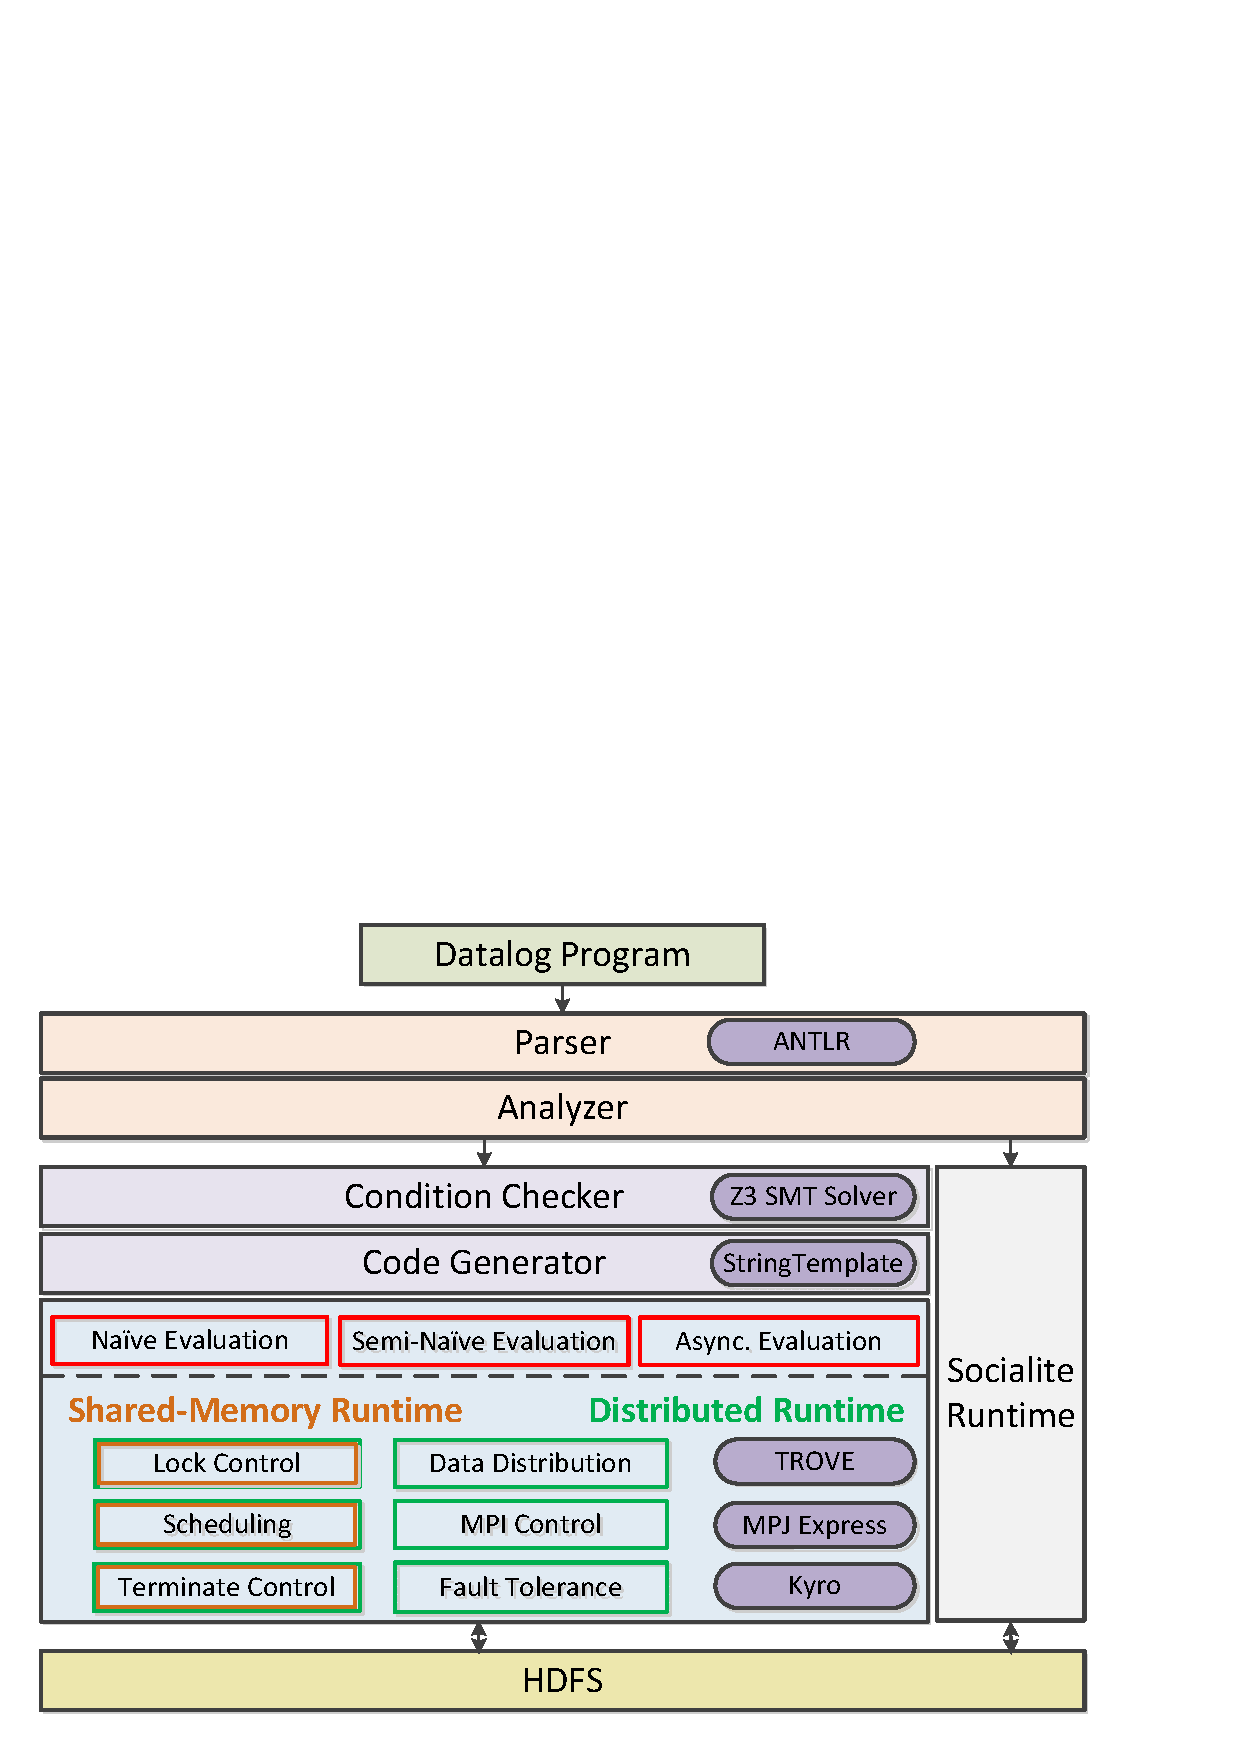
\includegraphics[width=3.2in]{fig/overview}
  \vspace{-0.1in}
  \caption{A3Log overview}
  \label{fig:overview}
  \vspace{-0.2in}
\end{figure}


A3Log is implemented using Java and contains several components as shown in Fig. \ref{fig:overview}. The \textbf{Parser} parses user's Datalog program into an abstract syntax tree (AST) by using ANTLR \cite{antlr}. The \textbf{Analyzer} traverses the AST to performs syntactic and semantic analysis, identifies the recursive rule, and analyzes the aggregate operation $g$ and non-aggregate operation $f$. If the program is a recursive program, it will be further processed by our system, otherwise it will be executed by the Socialite runtime engine \cite{Lam:2013:SDE:2510649.2511289,Seo:2013:DSD:2556549.2556572}. Given the $f$ and $g$ operations retrieved by the Analyzer, the \textbf{Condition Checker} relies on Z3 SMT Solver \cite{DeMoura:2008:ZES:1792734.1792766,z3} to verify the conditions and automatically chooses the appropriate evaluation technique. The \textbf{Code Generator} provides a series of code templates for generating the share-memory runtime code and distributed runtime code, where we use StringTemplate \cite{stringtemplate} to generate source code. Then, the recursive program will be executed by our execution engine (Sec. \ref{sec:system:runtime}). A3Log provides both \textbf{Shared-Memory Runtime Engine} and \textbf{Distributed Runtime Engine}. The shared-memory runtime and distributed runtime share several functionalities, including lock control, scheduling, termination check. The distributed runtime additionally supports data distribution, MPI control, and fault tolerance. We use TROVE \cite{trove} for high performance container operations which are frequently used due to our key table structure, use MPJ Express \cite{mpich} for MPI communication, and use Kryo \cite{kryo} for efficient serialization and deserialization. As implemented in Socialite, A3Log also relies on HDFS to store data and to checkpoint intermediate computation state.

\subsection{Datalog and Extension}
\label{sec:system:datalog}

A Datalog program is a set of rules. A \emph{rule} \texttt{r} has the form $h\leftarrow b_1,\ldots,b_n$, where $h$ is the \emph{head} and $b_1,\ldots,b_n$ is the \emph{body}. The comma separating literals in a body is a logical conjunction (AND). $h$ and $b_i$ can be with the form $p_i(t_1,\ldots,t_j)$ where $p_i$ is a \emph{predicate} and $t_1,\ldots,t_j$ are terms which can be \emph{constants}, \emph{variables} or \emph{functions}. For example, the Datalog program for SSSP computation can be written as follows.
%The data associated with abstract predicate is referred to as \emph{fact}.

\begin{verbatim}
  Program 1. Single Source Shortest Path
\end{verbatim}
\vspace{-0.1in}
\small
\begin{lstlisting}
  r1. sssp(X,$d$)$\leftarrow$ X=1,$d=0$.
  r2. sssp(Y,min[$d$])$\leftarrow$ sssp(X,$d1$),edge(X,Y,$d2$),
                       $d=d1+d2$,sssp(Y,$d$).
\end{lstlisting}
\normalsize

In Program 1, rule \texttt{r1} initializes the predicate \texttt{sssp} by specifying the source node $X=1$ and the shortest distance from source as $d=0$. \texttt{r2} is a recursive rule since it has the \texttt{sssp} predicate in both its head and body. \texttt{r2} will recursively produce \texttt{sssp} fact by joining the old \texttt{sssp} and \texttt{edge}. If there is a path from source to $X$ of length $d_1$ and an edge from $X$ to $Y$ of length $d_2$, there is a path from source to $Y$ with length $d=d_1+d_2$. If there is already a path to $Y$ found before, it should be also considered. Hence, the shortest distance from source to $Y$ is updated by the minimum of these possible distances, i.e., min$[d]$. The recursion will terminate as soon as no shortest distance is updated.

Originally, the Datalog program terminates when no new fact can be found. However, some programs will never stop since it continuously produces ``tiny'' facts. For example, the PageRank computation will continuously update the PageRank scores even though the changes are less and less. In order to help users express more termination conditions, we allow users to specify the termination conditions using aggregations.

\begin{verbatim}
  Program 2 PageRank
\end{verbatim}
\vspace{-0.1in}
\small
\begin{lstlisting}
  r1. degree(X,count[Y])$\leftarrow$ edge(X,Y).
  r2. rank(X,$r$) $\leftarrow$ node(X),$r=1$.
  r3. rank(Y,sum[$r$]+0.15) $\leftarrow$ rank(X,$r1$),edge(X,Y),
                            degree(X,$d$),
                            $r=0.85\cdot r1/d$,
                            [sum$[\Delta r]\leq 0.001$].
\end{lstlisting}
\normalsize

In Program 2, we show the Datalog program for PageRank. \texttt{r1} computes the node degrees based on the edge data. \texttt{r2} initializes the predicate \texttt{rank} by specifying all the nodes' ranking scores as a constant 1. \texttt{r3} is a recursive rule that updates the predicate \texttt{rank}. We allow users to specify the terminate conditions in $[\ldots]$ by using different aggregate operations. In this program, the PageRank computation will terminate when the sum of ranking score differences of two continuous recursion results is less than or equal to 0.001.

Besides SSSP and PageRank, we list 11 more example Datalog programs that can be executed asynchronously in the Appendix Sec. \ref{sec:app:example}. These examples cover a wide range of applications, including graph analytics (Program 3, 4, 5, 12), data mining (Program 6, 7, 9, 10), machine learning (Program 8, 11), and HPC (Program 13).

\subsection{Condition Checker}
\label{sec:system:condition}

\begin{figure}[!t]
    \centering
  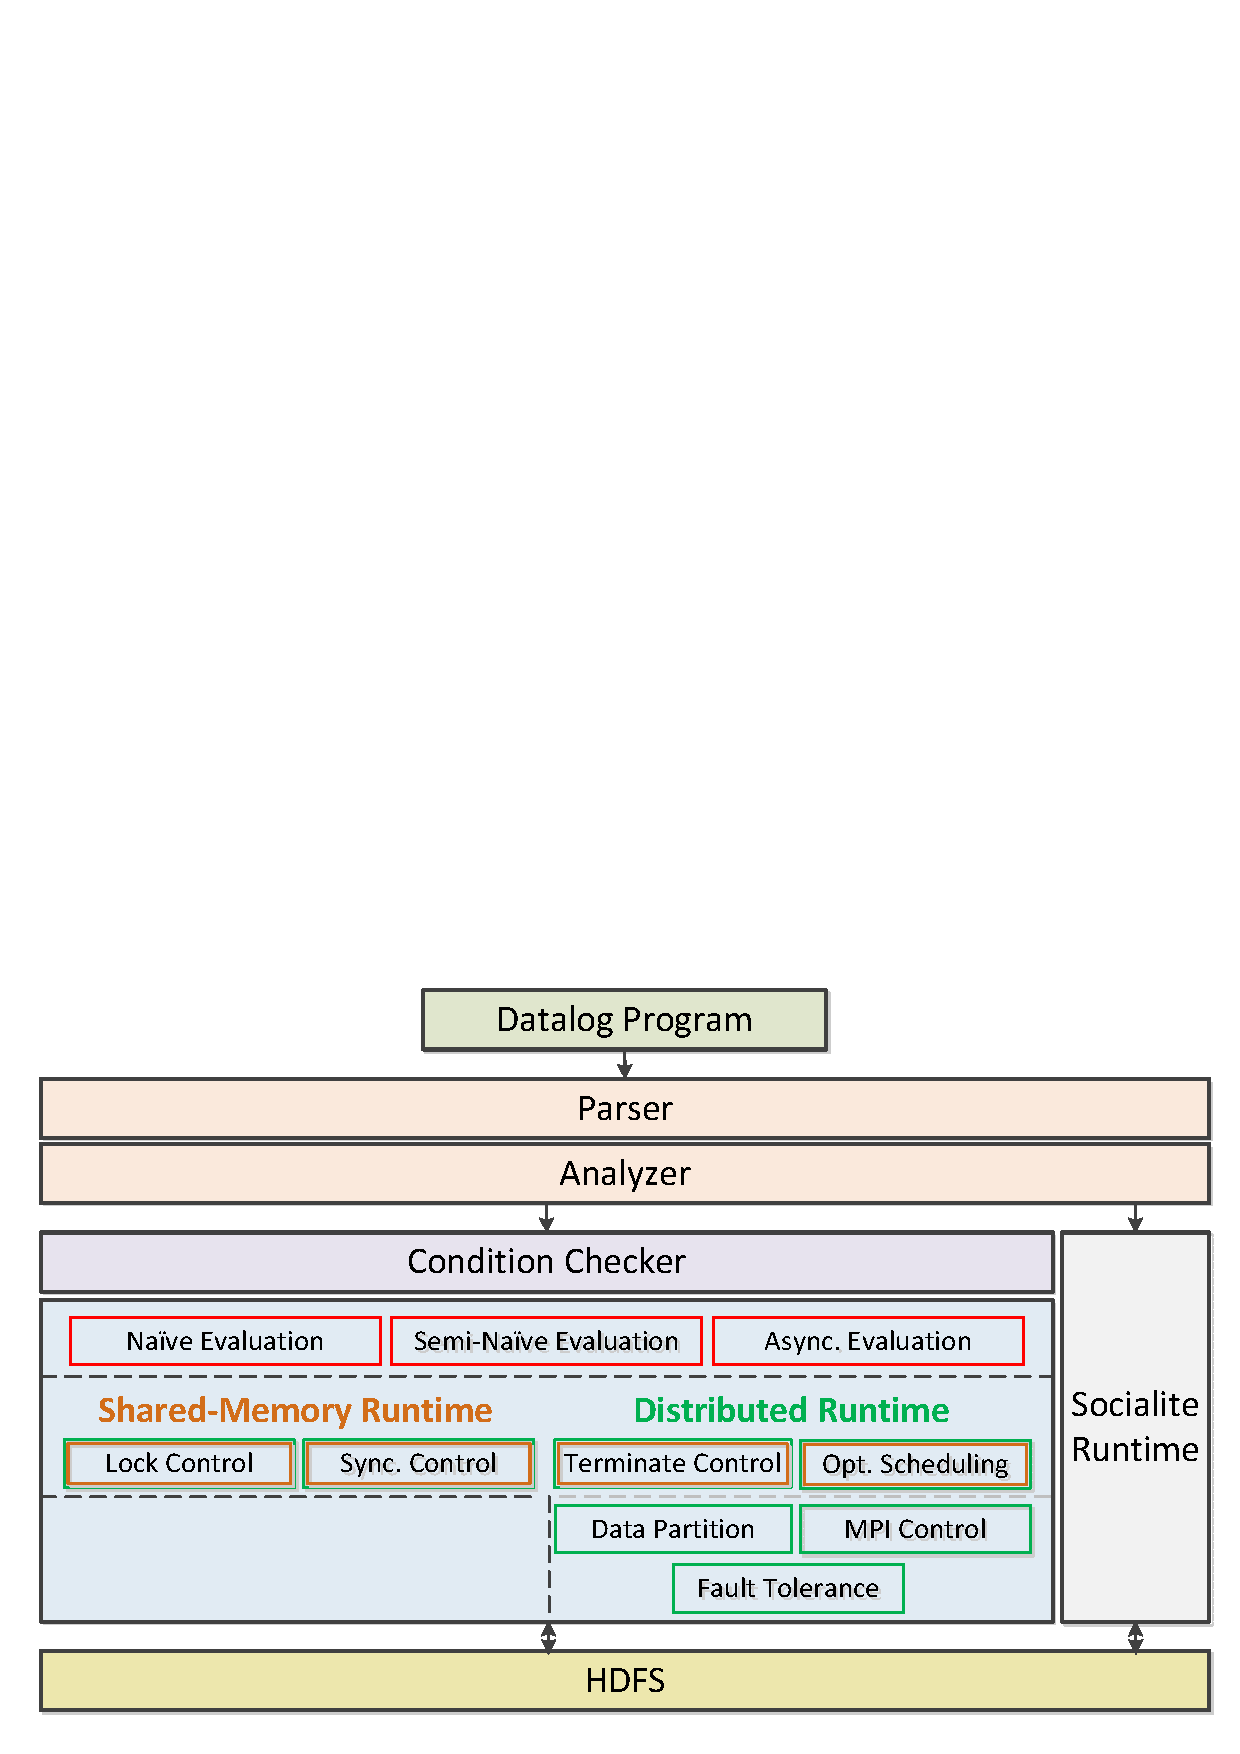
\includegraphics[width=2.8in]{fig/flow}
  \vspace{-0.1in}
  \caption{Condition checking flow chart}
  \label{fig:flow}
  \vspace{-0.2in}
\end{figure}

A3Log is able to automatically verify the conditions for asynchronous aggregation and accordingly selects the appropriate optimization technique according to the satisfiable conditions. The $g$ operation is identified as the update operation in the recursive rule's head predicate, e.g., min[$d$] in SSSP and sum[$r$]+0.15 in PageRank where [$d$] and [$r$] are the inputs, respectively. The $f$ operation is identified as the computation in the recursive rule's certain body predicate that updates the input variables of $g$ operation, e.g., $d=d1+d2$ in SSSP and $r=0.85\cdot r1/d$ in PageRank. The input variable of $f$ operation is the variable that appears in the recursive predicate, e.g., $d1$ in \texttt{sssp(X,$d1$)} and $r1$ in \texttt{rank(X,$r1$)}.

There are two techniques for executing recursive Datalog programs. The first is \emph{\textbf{Naive Evaluation}}. For instance, in Program 1, the recursive rule \texttt{r2} will be repeatedly evaluated. The \texttt{edge} facts keep being joined with the \texttt{sssp} facts discovered so far in each iteration, until no new fact is produced. This approach will inefficiently re-produce known facts in every iteration. To address this inefficiency issue, the \emph{\textbf{Semi-Naive Evaluation}} for recursive programs with aggregation was proposed \cite{Lam:2013:SDE:2510649.2511289,Wang:2015:AFR:2824032.2824052}, which is efficient and produces no duplicates. However, the semi-naive evaluation requires the program to be set-containment monotonic in order to guarantee the correctness. This is the same as the monotonizability condition that we have defined in Theorem \ref{th:monotone}. Therefore, as long as the program satisfies monotonizability condition or can be converted to be monotonic according to Theorem \ref{th:convert}, it can be executed with semi-naive evaluation. Furthermore, we propose \emph{\textbf{asynchronous evaluation}} as a yet another optimization technique, which allows asynchronous aggregation. We provide the sufficient conditions for asynchronous aggregation in Theorem \ref{th:async}. The prerequisite for asynchronous aggregation is the monotonic condition. Asynchronous evaluation is possible only when the recursive program is monotonic and satisfies order independent condition.

Condition Checker first translates the $f$ and $g$ operations into Z3 \cite{DeMoura:2008:ZES:1792734.1792766} satisfiability formulas (see Sec. \ref{sec:async:autoasync}). By applying $f$ and $g$ to the built-in condition checking templates, the Z3 SMT olver will answer satisfiable, unsatisfiable, or unknown. Following the condition checking flow as shown in Fig. \ref{fig:flow}, our system can automatically select the appropriate evaluation technique.

\subsection{Key Data Structure: AsyncTable}
\label{sec:system:data}

Before launching the recursive computation, the key table structure, AsyncTable, should be first prepared. AsyncTable maintains the computation states, which are initialized based on user's Datalog program and keeps being updated during the whole recursive computation process.

\begin{figure}[!t]
    \centering
  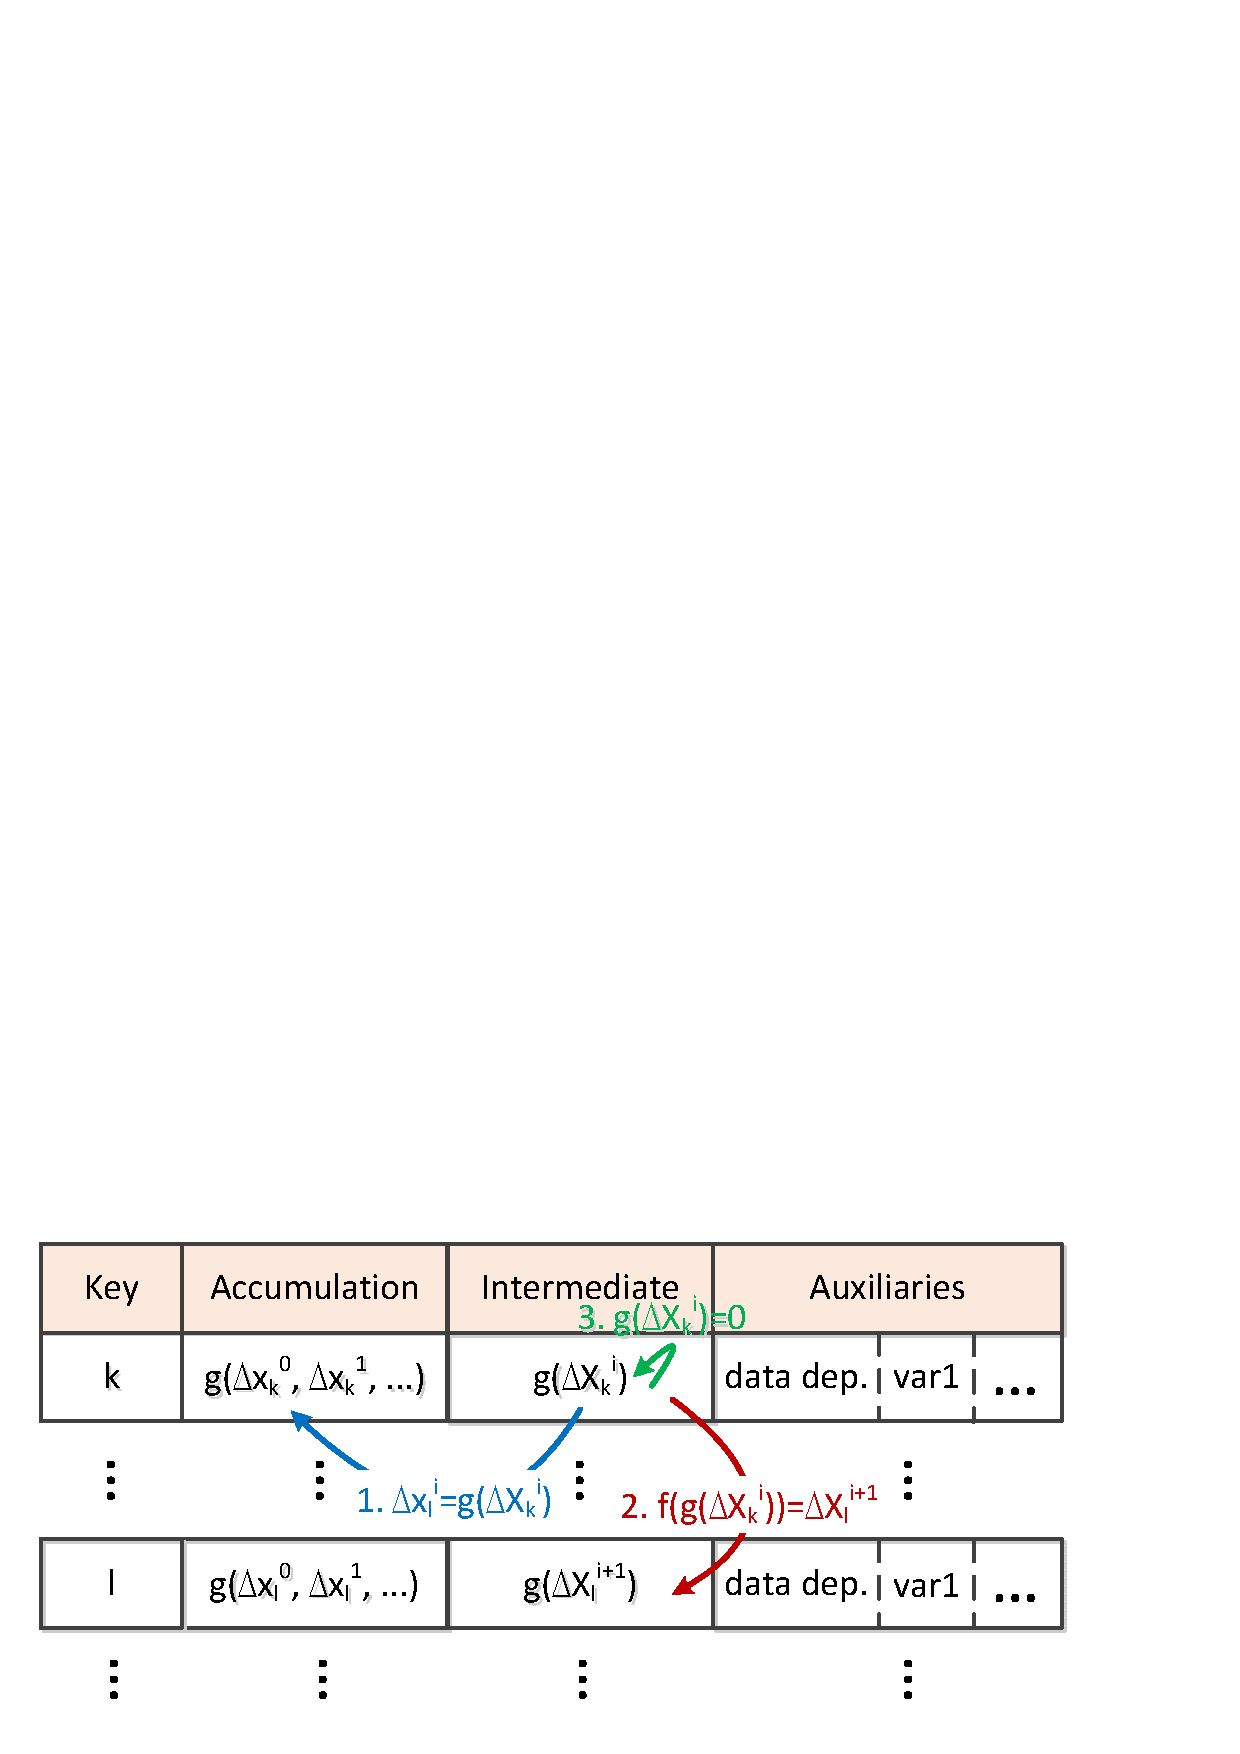
\includegraphics[width=3.2in]{fig/asynctable}
  \vspace{-0.1in}
  \caption{AsyncTable update}
  \label{fig:asynctable}
  \vspace{-0.2in}
\end{figure}

\Paragraph{AsyncTable Design}
As shown in Fig. \ref{fig:asynctable}, the AsyncTable contains several columns. The main key column and accumulation column store the result key-value pairs. The main key entries index the table. The accumulation column entry monotonically aggregates the intermediate results and maintains $g(\Delta x^0,\Delta x^1,\ldots)$. The accumulative property of $g$ operation makes it possible to use a single column to maintain all the intermediate results. The intermediate column entry stores the temporary aggregation results $g(\Delta X^k)$ which will be used to generate future intermediate results by applying $f$ operation. The auxiliary columns store the data which might be used by the $f$ or $g$ operation, e.g., outgoing neighbors set in SSSP and the node degree value in PageRank. The accumulation column entries and intermediate column entries are volatile, which maintain the computation states and keep being updated during the computation, while the other column entries are fixed after initialization. The AsyncTable is sharded for parallel processing. Each shard contains a number of rows and is assigned to a compute thread or placed on a distributed worker machine.

\Paragraph{AsyncTable Initialization}
The AsyncTable is initialized according to user's program. The recursive rule head contains the main key and accumulation column's information. For example in SSSP, the main key column entries are initialized with the node ids. The accumulation column is initialized with the identity element \textbf{0} w.r.t $g$, e.g., MAX in SSSP. The intermediate column is initialized in terms of the non-recursive rule \texttt{r1}, i.e., 0 for the source node and MAX for other nodes. The auxiliary data dependency column is identified as the rule body predicate that describes the relationship between main keys, e.g., \texttt{edge(X,Y,d2)}. The auxiliary variable column entries can be identified as the joined results between rule body predicates, e.g., the degree information \texttt{d} in PageRank.

A few additional facts should be noticed: 1) It is possible that two or more items are identified as the main key (see Program 4, 5, and 12 in Appendix Sec. \ref{sec:app:example}); 2) The AsyncTable size can be dynamic rather than fixed due to the continuously inserted new rows (see Program 4, 5, 7, and 9); 3) The recursive program can be composed of more than one interdependent rules, which can be reduced to one rule (see Program 9 and 10).

%\Paragraph{AsyncTable Sharding and Distribution}
%Each \emph{shard} contains a number of rows and is assigned to a compute thread in shared-memory runtime or placed on a worker machine in distributed runtime. There are two kinds of sharding: range-based and hash-based. A3Log prefers the hash sharding since it is adaptable to the case that the rows are dynamically inserted.

\subsection{Execution Runtime Engine}
\label{sec:system:runtime}

\begin{figure}[!t]
    \centering
  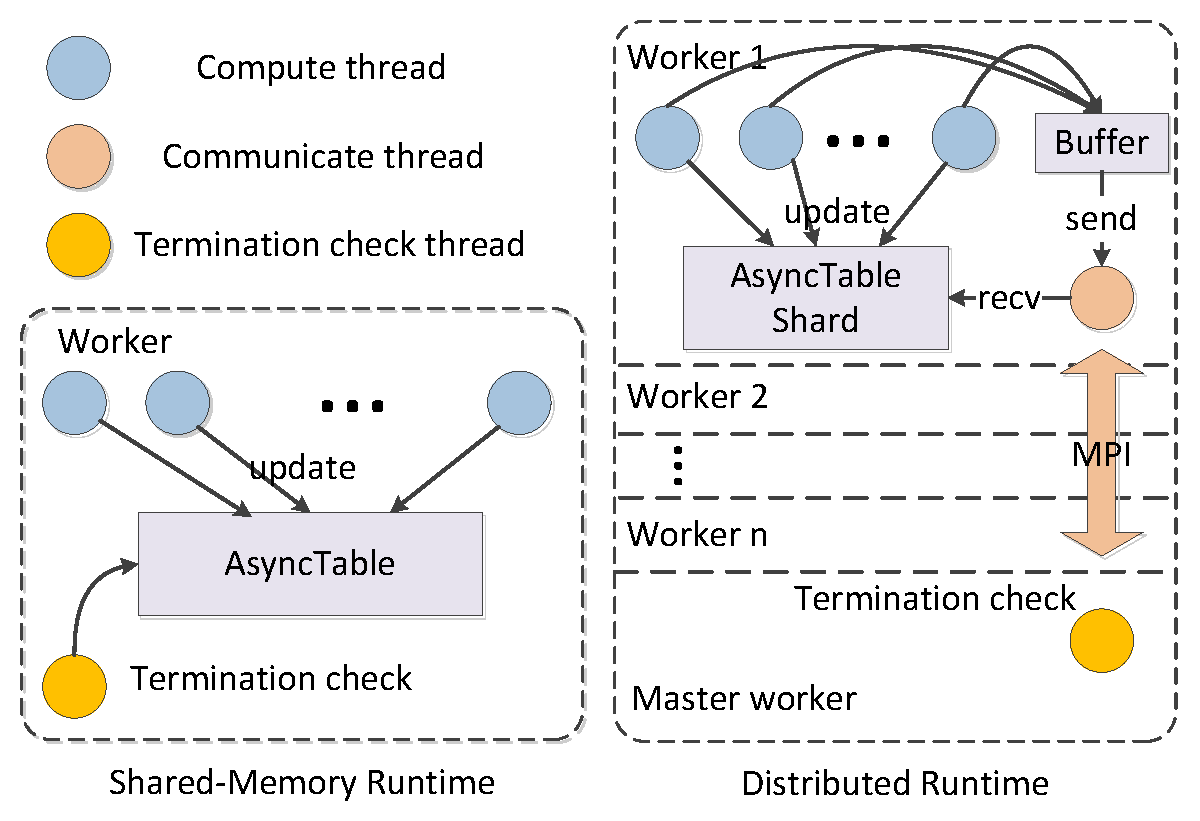
\includegraphics[width=2.9in]{fig/runtime}
  \vspace{-0.1in}
  \caption{Execution Runtime Engine}
  \label{fig:runtime}
  \vspace{-0.1in}
\end{figure}

\Paragraph{Overall Architecture}
A3Log provides both shared-memory runtime engine and distributed runtime engine. Fig. \ref{fig:runtime} shows the overall structure. The shared-memory runtime has a simple design. A number of compute threads are created to update the AsyncTable in parallel, and a termination check thread is running separately to check the stop condition. The distributed runtime contains a number of workers and a master worker. Each worker creates a number of compute threads to update the local AsyncTable shard. A communicate thread tackles the remote update. We adopt a send buffer design to control the overhead of frequent communications. The master worker creates a termination check thread to globally check stop condition periodically.

%Our \emph{Code Generator} will generate the shared-memory runtime code and distributed runtime code based on a set of code templates. They will then be compiled and run on runtime engines.

\Paragraph{Concurrency Control}
The accumulation column entries and intermediate column entries keep being updated during computation. Specifically, an intermediate column entry is read to update the same row's accumulation column entry (by operation 1 in Fig. \ref{fig:asynctable}) and to update other rows' intermediate column entries (by operation 2 in Fig. \ref{fig:asynctable}), and is reset as \textbf{0} (by operation 3 in Fig. \ref{fig:asynctable}). The reset operation is essential to make result correct, without which the same intermediate result would be redundantly accumulated. These three operations have to be \emph{atomic} according to the definition of accumulated recursive program (Definition \ref{eq:accumasync}). However, an intermediate column entry can be read and written concurrently by multiple threads or multiple workers, which leads to potential consistency problem. In our shared-memory runtime, we use \emph{optimistic} lock to avoid read-write conflicts. In distributed runtime, the consistency problem will happen in the send buffer, which maintains the remote updates. The optimistic lock does not work well since the communicate thread is required to serialize the whole buffer for efficiency and the lock granularity becomes too coarse to result in too many aborts. We employ MVCC (multi-version concurrency control) to address this problem. Specifically, we adopt a double-version design of the send buffer, which serves the compute threads and communicate thread alternatively.

%In our distributed runtime, we have a send buffer design to avoid frequent communications where the buffered messages will be serialized and sent out together. As shown in Fig. \ref{fig:runtime}, the compute threads write messages to the buffer that are the remote updates (i.e., operation 2 in Fig. \ref{fig:asynctable}), and the communicate thread sends out the whole buffered messages and clears up the buffer (i.e., operation 3 in Fig. \ref{fig:asynctable}). The consistency problem still exists with the buffer design. Unfortunately, the optimistic lock will not work since the whole buffer is the basic operation unit by the communicate thread where the lock granularity is too coarse to result in too many aborts. We propose a \emph{swing buffer} design that maintains two versions of the buffer, one for compute thread and one for communicate thread. After the communicate thread has processed and cleared up one buffer, it is switched to process the other buffer with full of messages filled by the compute thread. At the same time the compute thread switches to write messages to the buffer that is cleared up by the communicate thread. In this way, neither read-write conflicts nor write-write conflicts exist. Fundamentally speaking, we use \emph{optimistic concurrency control} (OCC) in shared-memory runtime and \emph{multi-version concurrency control} (MVCC) in distributed runtime to solve the consistency problem.


\Paragraph{Scheduling}
As discussed in Sec. \ref{sec:async:pri}, the clever scheduling of aggregate operations has the potential of accelerating the convergence of recursive computations. The scheduling should be performed by evaluating the intermediate aggregation result (intermediate column entries in AsyncTable). The top intermediate column entries (in the partial order defined by $g$) should be scheduled. Since the intermediate column entries keep being updated, the top entries should be evaluated frequently. For the sake of reducing scheduling cost, we utilize the sampling technique \cite{Zhang:2011:PDF:2038916.2038929} to approximately obtain the top $N\%$ entries. The scheduling is even more costly in distributed environment. Rather than global scheduling, local scheduling in each worker is preferred.
%The portion ($N\%$) of entries to be scheduled balances the tradeoff between the optimal scheduling benefit and the sorting cost. We will empirically study the effect of $N\%$ in Sec. \ref{sec:expr:schedle}.

\Paragraph{Termination Check}
The termination condition might rely on aggregation of either the accumulation column entries or the intermediate column entries. The aggregation is evaluated by the termination check thread without disturbing the compute threads. While in distributed runtime, each worker will report their local aggregation results to the master, where the global termination check thread determines whether to stop by evaluating the global aggregation result. Note that, there is no iteration's conception in asynchronous aggregation, so we have to check the termination condition every other period of time rather than every other iteration.

%In shared-memory runtime, a termination check thread periodically checks the user specified termination condition.

\Paragraph{Fault Tolerance}
For large scale operations that involve many machines for a substantial amount of time, it is also important to provide fault tolerance support. A3Log relies on Socialite's fault tolerance scheme \cite{Seo:2013:DSD:2556549.2556572}. The intermediate computation states are checkpointed occasionally on HDFS and restorable as needed. If one or more workers fail, the intermediate states are restored from the latest checkpoint and the evaluation is resumed from that point.

















\begin{comment}
\subsection{New Recursive Datalog Programs with Delta-Aggregate Operation}

\begin{verbatim}
  Program 1. Single Source Shortest Path
\end{verbatim}
\vspace{-0.12in}\small
\begin{lstlisting}
  r1. sssp(X,dmin[$\Delta d$])$\leftarrow$ X=1,$\Delta d=0$.
  r2. sssp(Y,dmin[$\Delta d$])$\leftarrow$ sssp(X,$\Delta d1$),
                         edge(X,Y,$d2$),
                         $\Delta d=\Delta d1+d2$.
\end{lstlisting}
\normalsize

\begin{verbatim}
  Program 2. PageRank
\end{verbatim}
\vspace{-0.12in}\small
\begin{lstlisting}
  r1. degree(X,count[Y])$\leftarrow$ edge(X,Y).
  r2. pagerank(X,dsum($\Delta r$)) $\leftarrow$ node(X),$\Delta r=1-\lambda$.
  r3. pagerank(Y,dsum[$\Delta r$]) $\leftarrow$ edge(X,Y),
                              pagerank(X,$\Delta r1$),
                              degree(X,$d$),
                              $\Delta r=\lambda\cdot \Delta r1/d$,
                              $\Delta r \geq 0.00001$.
\end{lstlisting}
\normalsize


\begin{verbatim}
  Program 3. Connected Conponents
\end{verbatim}
\vspace{-0.12in}\small
\begin{lstlisting}
  r1. cc(X,dmin(X))$\leftarrow$ edge(X,_).
  r2. cc(Y,dmin[$\Delta v$])$\leftarrow$ cc(X,$\Delta v$), edge(X,Y)
\end{lstlisting}
\normalsize

\begin{verbatim}
  Program 4. Computing Paths in a DAG
\end{verbatim}
\vspace{-0.12in}\small
\begin{lstlisting}
  r1. cpaths(X,Y,dcount(1)) $\leftarrow$ edge(X,Y).
  r2. cpaths(X,Y,dcount[$\Delta c$]) $\leftarrow$ cpaths(X,Z,$\Delta c$),
                                edges(Z,Y)
\end{lstlisting}
\normalsize
will show a step-by-step example in figure


\begin{verbatim}
  Program 5. Max Probability Path
\end{verbatim}
\vspace{-0.12in}\small
\begin{lstlisting}
  r1. reach(X,Y,dmax($P$)) $\leftarrow$ net(X,Y,$P$).
  r2. reach(X,Y,dmax[$\Delta P$]) $\leftarrow$ reach(X,Z,$\Delta P1$),
                             reach(Z,Y,$\Delta P2$),
                             $\Delta P=\Delta P1*\Delta P2$.
\end{lstlisting}
\normalsize


\begin{verbatim}
  Program 6. Least Common Ancestor
\end{verbatim}
\vspace{-0.12in}\small
\begin{lstlisting}
  r1. ancestor(Y,X,dmin(1)) $\leftarrow$ cite(Y,X), X<seed.
  r2. ancestor(Z,X,dmin[$\Delta d+1$]) $\leftarrow$ ancestor(Z,Y,$\Delta d$),
                                    cite(Y,X).
  r3. LCA(p1,p2,min[max(  $\leftarrow$ ancestor(p1,X,d1),
        d1,d2)],year,X)      ancestor(p2,X,d2),
                             Paper(X,year),
                             p1<p2.
\end{lstlisting}
\normalsize

\begin{verbatim}
  Program 7. What is the cost of each part
\end{verbatim}
\vspace{-0.12in}\small
\begin{lstlisting}
  r1. cost(Part,dsum($c$)) $\leftarrow$ basic(Part,cost).
  r2. cost(Part,dsum[$\Delta \mathcal{C}$]) $\leftarrow$ assb(Part,Sub,$n$),
                            cost(Sub,$\Delta c$),
                            $\Delta \mathcal{C}=\Delta c*n$.
\end{lstlisting}
\normalsize

Program 7 is for computing the cost of a part from the cost of its subparts, respectively. The \texttt{assb} predicate denotes each part��s required subparts and number required and basic denotes the number of days for a part to be received and the part��s cost.

\begin{verbatim}
  Program 8. Viterbi Algorithm
\end{verbatim}
\vspace{-0.12in}\small
\begin{lstlisting}
  r1. calcV(0,X,dmax($L$)) $\leftarrow$ s(0,EX),p(X,EX,$L1$),
                            pi(X,$L2$),$L=L1*L2$.
  r2. calcV($T$,Y,dmax[$\Delta L$]) $\leftarrow$ s($T$,EY),p(Y,EY,$L1$),
                            $T1=T-1$,t(X,Y,$L2$),
                            calcV($T1$,X,$\Delta L3$),
                            $\Delta L=L1*L2*\Delta L3$.
\end{lstlisting}
\normalsize

\begin{verbatim}
  Program 9. Who will come to the party?
\end{verbatim}
\vspace{-0.12in}\small
\begin{lstlisting}
  r1. coming(X) $\leftarrow$ sure(X).
  r2. coming(X) $\leftarrow$ cntComing(X,$N$), $N\geq 3$.
  r3. cntComing(Y,dcount[*]) $\leftarrow$ friend(Y,X),
                                coming(X).
\end{lstlisting}
\normalsize

\begin{verbatim}
  Program 10. Galaxy Evolution
\end{verbatim}
\vspace{-0.12in}\small
\begin{lstlisting}
  r1. galaxies(1,gid) $\leftarrow$ galaxies_seed(gid).
  r2. galaxies(t+1,gid2) $\leftarrow$ galaxies(t,gid1),
                            edges(t,gid1,gid2,c),
                            c$\geq$threshold.
  r3. edges(t,gid1,gid2, $\leftarrow$ galaxies(t,gid1),
        dcount[*])          particles(pid,gid1,t),
                            particles(pid,gid2,t+1).
\end{lstlisting}
\normalsize
\end{comment}

\section{Performance Evaluation}
\label{sec:expr}

We empirically evaluate A3Log on Amazon EC2. We will show the comparison results with other systems, with different algorithms, and with different datasets. More experimental results can be found in Appendix Sec. \ref{sec:app:expr}, including scaling performance and effectiveness of aggregations.


%A3Log provides both shared-memory runtime and distributed runtime.
%with the state-of-the-art parallel/distributed frameworks in the context of different workloads in this section.



\subsection{Comparison to Other Systems}
\label{sec:expr:othersystems}

\Paragraph{Competitors}
A3Log is compared with four state-of-the-art parallel/distributed frameworks. \textbf{SociaLite} \cite{Lam:2013:SDE:2510649.2511289,Seo:2013:DSD:2556549.2556572} is a Datalog implementation for social network analysis. \textbf{Myria} \cite{Halperin:2014:DMB:2588555.2594530,Wang:2015:AFR:2824032.2824052} supports Datalog asynchronous evaluation. Both SociaLite and Myria support monotonic aggregation inside recursion. \textbf{GraphLab} \cite{Low:2012:DGF:2212351.2212354} is a graph-based parallel/distributed engine supporting asynchronous iteration. \textbf{Maiter} \cite{maiter} supports delta-based accumulative iterative computation (similar to monotonic aggregation) which can be executed asynchronously. All these systems are configured with their default parameters. Myria, GraphLab, and Maiter are configured to run with asynchronous model unless particularly mentioned. The runtime results are the execution time excluding data loading time, and each is a mean of two runs.

%Socialite also supports COST computation, and Myria also supports LCA computation.

%We first compare A3Log with the other state-of-the-art systems in the context of seven algorithms. In order to see the benefit from asynchronous aggregation and eliminate the interference from system implementation factors, we also implement a synchronous version of A3Log, i.e., \textbf{A3Log(sync.)}, for comparison.
\Paragraph{Algorithms and Datasets}
We compare A3Log with other systems in the context of three algorithms, including SSSP (Program 1), PageRank (Program 2), and Connected Components (CC, Program 3). These three algorithms are all supported by these systems. For SSSP and CC, the computations terminate as soon as no new update is found. For PageRank in A3Log and Maiter, which has no notion of iterations, the computation terminates when the sum of difference to the theoretical convergence point \cite{Zhang:2011:PDF:2038916.2038929} is less than $10^{-4}$ (see Appendix Sec. \ref{sec:expr:aggregations}), based on which we know the number of iterations that is required to reach the same point (42 iterations) \cite{Zhang:2011:PDF:2038916.2038929}. Socialite and Myria (Myria does not support asynchronous PageRank) are set to run 42 iterations. GraphLab terminates after the PageRank value of every vertex changes by less than a user-specified threshold $\epsilon$ between two consecutive executions of that vertex. These algorithms are performed on a large graph dataset ClueWeb09 \cite{clueweb}. In order to finish the experiments in a reasonable time, we truncate the original dataset into a smaller ClueWeb20M dataset with 20,000,000 nodes, 243,063,334 edges, and 3.8GB size. Since ClueWeb is an unweighted graph, we assign a random weight to each edge for SSSP computation.



\begin{figure}[!t]
\vspace{-0.1in}
    \centering
  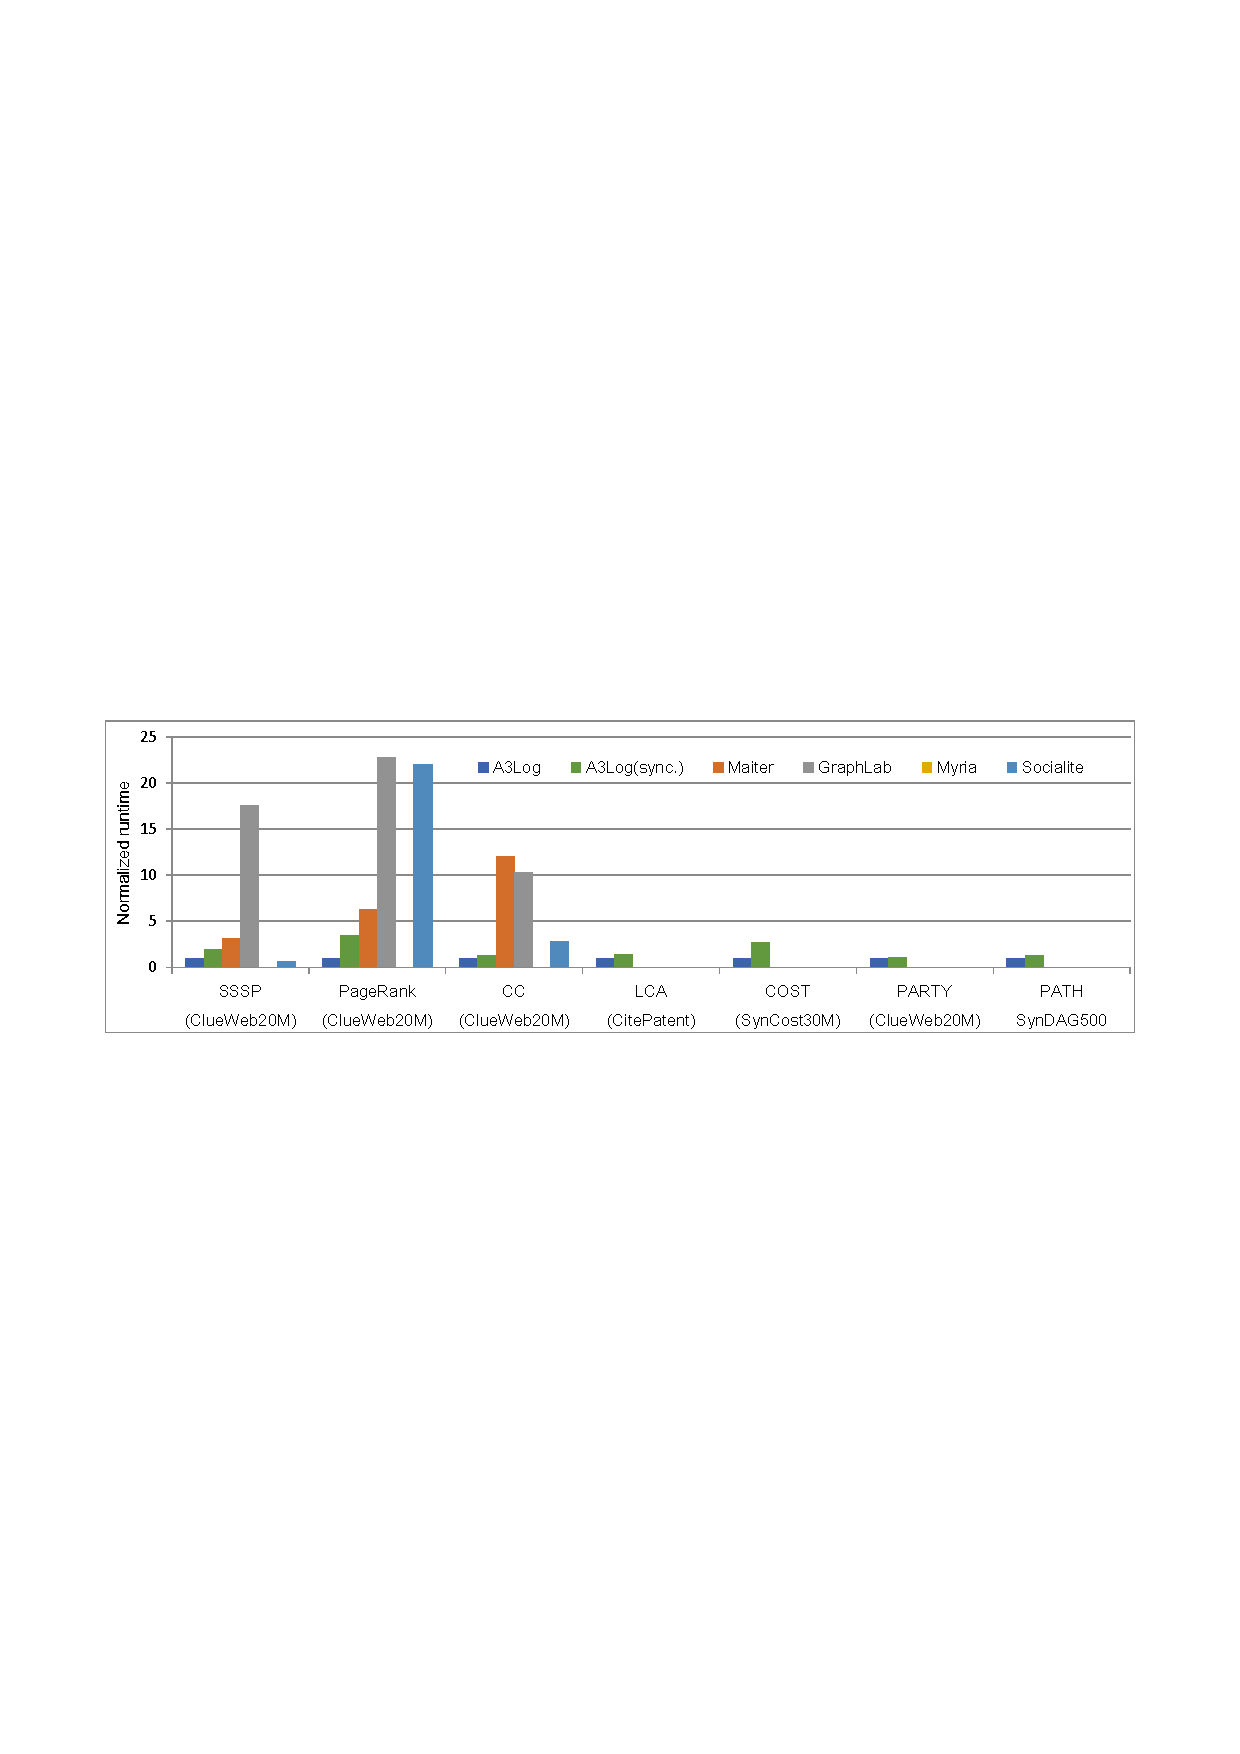
\includegraphics[width=3in]{fig/single-result}
  \vspace{-0.1in}
  \caption{Performance comparison with other systems (many-core environment)}
  \label{fig:single-result}
  \vspace{-0.2in}
\end{figure}

%myria exclude the loading time
%when to converge, fix iteration num

In the shared-memory experiment, we run all the systems on an r3.8xlarge EC2 instance with 32 vCPUs and 244GB memory. We configured all these systems with 32 threads. The normalized runtime results. In general, A3Log outperforms all the competitors. For the PageRank computation, A3Log achieves 22.8X speedup over GraphLab, 22X speedup over Socialite, 6X speedup over Maiter, and much more speedup over Myria\footnote{The runtime results of Myria may be wrong because they are all unexpected long, say 135 times longer for PageRank and 321 times longer for SSSP than A3Log. We are contacting with Myria authors to fix it but cannot find the problem before the submission.} are shown in Fig. \ref{fig:single-result}. There is an exception for SSSP computation. Socialite is 1.6X faster than A3Log. This may be due to their \emph{prioritization} optimization, which is similar to our scheduling technique that leads to Dijkstra algorithm.

%With different configurations, we see comparable performance with Socialite on SSSP computation. In addition, A3Log outperforms A3Log(sync) on all the applications.


\begin{figure}[!t]
\vspace{-0.1in}
    \centering
  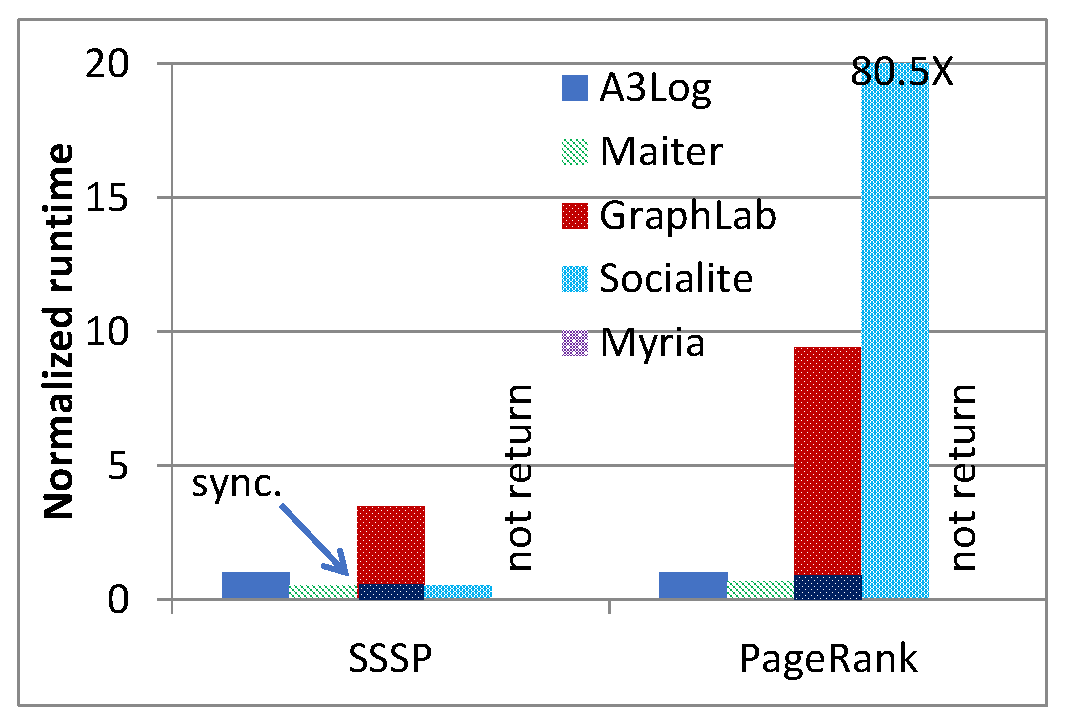
\includegraphics[width=2.4in]{fig/dist-result}
  \vspace{-0.1in}
  \caption{Performance comparison with other systems (distributed environment)}
  \label{fig:dist-result}
  \vspace{-0.2in}
\end{figure}

In the distributed experiment, we deploy all the systems on an EC2 cluster with 64 c4.2xlarge EC2 instances, each with 8 vCPUs and 15GB memory. The network bandwidth between instance workers is 10Gb/s\footnote{The network specification does not clearly describe the bandwidth but is only classified as \emph{High}, which is estimated as 10Gb/s.}. We configured all these systems with 8 threads for each worker. The normalized runtime results of SSSP and PageRank are shown in Fig. \ref{fig:dist-result}. A3Log outperforms GraphLab and Socialite on PageRank computation. The synchronous version of GraphLab performs much better than asynchronous GraphLab, which is due to its costly distributed locking \cite{Han:2015:GUB:2777598.2777604,Low:2012:DGF:2212351.2212354}. Socialite performs SSSP faster. The distributed Myria runs unexpected long without returning results, say 9 hours for PageRank and did not return. The performance of A3Log and Maiter is comparable on these two applications. The reason why A3Log does not show significant better performance in distributed environment is because of the expensive communication overhead. The communication module relies on a pure Java implementation of MPI, MPJ express \cite{mpich}, which shows about 10 times lower performance than native C implementation of Open MPI \cite{mpjperformance}. We adopt MPJ for its good compatibility but at the expense of performance. We are implementing an alternative distributed runtime based on Open MPI \cite{openmpi}.


\subsection{Performance Gain Analysis}
\label{sec:expr:optimizations}

\begin{figure}[!t]
    \centering
  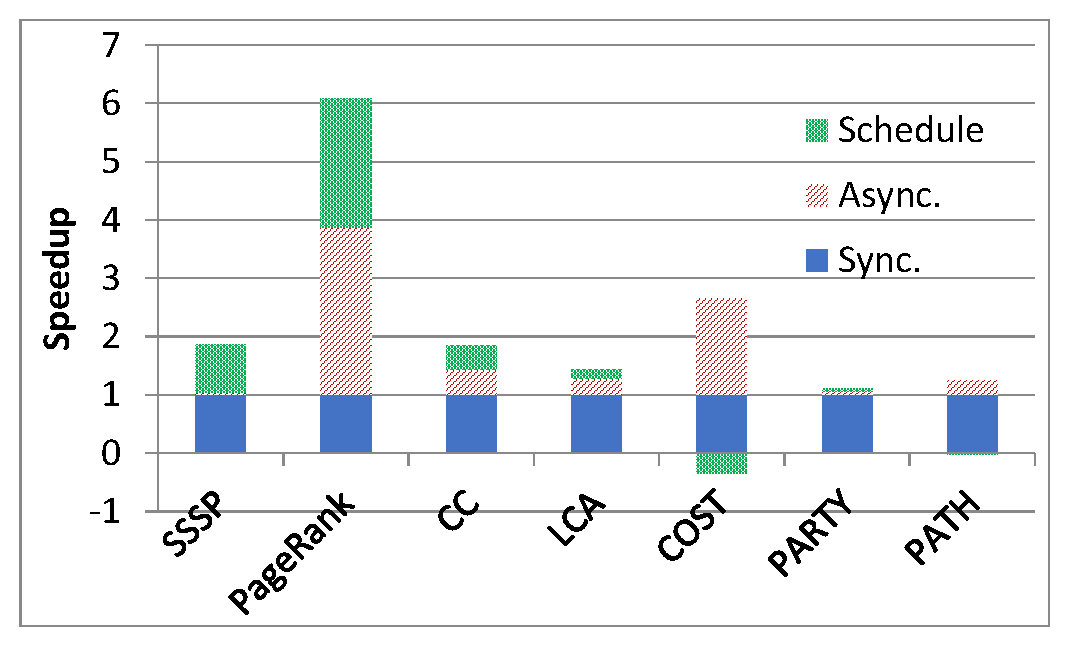
\includegraphics[width=2.8in]{fig/single-optimize}
  \caption{Performance gain analysis}
  \label{fig:single-optimize}
  \vspace{-0.2in}
\end{figure}

\begin{table*}[!t]
%\vspace{-0.1in}
    \caption{Performance when varying workloads (shared-memory runtime, $d$ is diameter, $e$ is powerlaw exponent)}
    \vspace{-0.1in}
    \label{tab:wrokload}
    \centering
    \small
    \begin{tabular}{c|c|c|c|c|c|c|c|c|c|c|c}
    \hline
 \multirow{2}{*}{\textbf{Dataset}} & \multirow{2}{*}{\tabincell{c}{\textbf{Nodes}}} & \multirow{2}{*}{\tabincell{c}{\textbf{Edges}}} & \multirow{2}{*}{\tabincell{c}{\textbf{Graph}\\ \textbf{type}}} & \multirow{2}{*}{\tabincell{c}{\textbf{$d$}}}& \multirow{2}{*}{\tabincell{c}{\textbf{$e$}}} & \multicolumn{3}{|c}{\textbf{SSSP}} & \multicolumn{3}{|c}{\textbf{PageRank}} \\
 \cline{7-12}
     &  & & & & & \textbf{Sync.} & \textbf{Async.} & \footnotesize{\textbf{Speedup}} & \textbf{Sync.} & \textbf{Async.} & \footnotesize{\textbf{Speedup}}\\
\hline\hline
\textbf{Actor} & 382,219 & 33,115,812 & \footnotesize{collaborate} & 13 & 2.131 & 34.62s & 1.54s & 22.44X & 63.62s & 7.03s & 9.05X \\
\hline
\textbf{Amazon} & 403,394 & 3,387,388 & \footnotesize{co-purchase} & 25 & 3.151 & 79.18s & 1.55s & 51.05X & 53.77s & 1.02s & 52.9X \\
\hline
\textbf{arXiv} & 28,093 & 4,596,803 & co-author & 9 & 1.731 & 19.7s & 1.51s & 13.03X & 53.2s & 1.01s & 52.7X \\
\hline
\textbf{DBLP} & 1,314,050 & 18,986,618 & co-author & 24 & 3.221 & 55.38s & 3.18s & 17.41X & 89.76s & 5.06s & 17.75X \\
\hline
\textbf{Flicker} & 2,302,925 & 33,140,017 & social & 23 & 1.711 & 38.3s & 3.95s & 9.71X & 84.24s & 24.2s & 3.48X \\
\hline
\textbf{Livejournal} & 5,204,176 & 49,174,464 & social & 23 & 1.537 & 57.26s & 9.41s & 6.08X & 111.09s & 49.43s & \textcolor{blue}{\textbf{2.25X}} \\
\hline
\textbf{Orkut} & 3,072,441 & 117,184,899 & social & 10 & 1.272 & 58.99s & 14.07s & \textcolor{blue}{\textbf{4.19X}} & 187.74s & 16.18s & 11.6X \\
\hline
\textbf{Patent-US} & 3,774,768 & 16,518,947 & citation & 26 & 4.001 & 66.83s & 3.21s & 20.8X & 68.06s & 6.11s & 11.15X \\
\hline
\textbf{Prosper} & 89,269 & 3,394,979 & loan & 8 & 2.191 & 37.75s & 1.51s & 24.93X & 52.61s & 1.02s & 51.58X \\
\hline
\textbf{RoadCA} & 1,965,206 & 2,766,607 & road net & 865 & 8.991 & 140.43s & 1.55s & 90.31X & 57.06s & 1.03s & \textcolor{red}{\textbf{55.59X}} \\
\hline
\textbf{RoadTX} & 1,379,917 & 1,921,660 & road net & 1064 & 8.901 & 137.2s & 1.55s & 88.4X & 54.49s & 1.02s & 53.63X \\
\hline
\textbf{Skitter} & 1,696,415 & 11,095,298 & Internet & 31 & 2.291 & 31.09s & 1.55s & 20.01X & 59.51s & 3.04s & 19.56X \\
\hline
\textbf{soc-LiveJ} & 4,847,571 & 68,475,391 & social & 20 & 2.651 & 67.2s & 11.2s & 6X & 113.51s & 39.2s & 2.9X \\
\hline
\textbf{soc-Pokec} & 1,632,803 & 30,622,564 & social & 14 & 3.081 & 53.85s & 4.81s & 11.19X & 76.83s & 15.1s & 5.09X \\
\hline
\textbf{TREC} & 1,601,787 & 8,063,026 & web & 112 & 2.231 & 130.84s & 1.6s & 81.62X & 55.29s & 2.03s & 27.23X \\
\hline
\textbf{\footnotesize{web-BerkStan}} & 685,230 & 7,600,595 & web & 208 & 2.601 & 692.08s & 3.1s & \textcolor{red}{\textbf{222.82X}} & 54.13s & 2.02s & 26.76X \\
\hline
\textbf{web-Google} & 875,713 & 5,105,039 & web & 24 & 2.731 & 70.8s & 1.59s & 44.64X & 54.24s & 2.03s & 26.67X \\
\hline
\textbf{Wiki-Talk} & 2,987,535 & 24,981,163 & \footnotesize{communicate} & 9 & 1.811 & 23.81s & 3.1s & 7.68X & 83.57s & 28.27s & 2.96X \\
\hline
\textbf{Youtube-u} & 3,223,589  & 9,375,374 & social & 31 & 2.211 & 30.6s & 2.43s & 12.6X & 65.91s & 5.08s & 12.96X \\
\hline
\textbf{\footnotesize{Zhishi-Baidu}} & 2,141,300 & 17,794,839 & web & 20 & 2.291 & 49.19s & 3.29s & 14.96X & 66.72s & 8.09s & 8.25X\\
\hline
\end{tabular}
\vspace{-0.1in}
\end{table*}

In order to analyze the factors for performance improvement and eliminate the interference from system implementation factors, we also implement a synchronous version of A3Log, which uses synchronous semi-naive evaluation (i.e., synchronous accumulated recursive programs). In addition, we turn off the scheduling then it shows the performance ahieved by pure asynchronous aggregation.

\Paragraph{Algorithms and Datasets}
We test more algorithms to see the effect variations on different workloads, including Least Common Ancestor (LCA, Program 6), ``What is the cost of each part?'' (COST, Program 7), ``Who will come to the party?'' (PARTY, Program 9), and ``Computing Paths in a DAG'' (PATH, Program 4). More details of these algorithms can be found in Appendix Sec. \ref{sec:app:example}. For LCA, we use a citation network Patent-US \cite{konect}. For COST, we synthetically generate a hierarchical (tree-like) dataset with 30,000,000 tree nodes. PARTY is a graph based algorithm, so we use the same ClueWeb20M dataset. For PATH, we synthetically generate a directed acyclic graph (DAG) dataset with 500 nodes and 35,952 edges. PATH is a computation intensive workload since it evaluates the paths between all pairs.


We run these algorithms on the an r3.8xlarge EC2 instance with 32 vCPUs and 244GB memory. All these experiments are run with 32 threads. Fig. \ref{fig:single-optimize} shows the results. The runtime by synchronous semi-naive evaluation is considered as the baseline. The speedups from asynchronous execution and prioritized scheduling exhibit variations for different workloads. Generally speaking, the graph based algorithms benefit from asynchronous aggregation and priority scheduling more. For SSSP and PageRank, great performance gains are achieved by priority scheduling. However, for COST, the priority scheduling brings negative effect. This is because that COST aims to compute all parts' cost in a hierarchical structure and the computations on these parts equally contribute to the output. Using priority scheduling will not bring any benefit but only incurs scheduling overhead. However, we still take advantage of asynchronous aggregation to avoid synchronizations and achieve better performance.


\subsection{Comparison with Different Workloads}
\label{sec:expr:workloads}


%Google \cite{google}, Livejournal \cite{livejournal}, RoadCA \cite{roadca}, WikiTalk \cite{wikitalk}



\begin{comment}
\begin{table*}[!htb]
    \caption{Performance when varying workloads (distributed runtime)}
    \vspace{-0.1in}
    \label{tab:wrokload}
    \centering
    \footnotesize
    \begin{tabular}{c|c|c|c|c|c|c|c|c|c|c|c}
    \hline
 \multirow{2}{*}{\textbf{Dataset}} & \multirow{2}{*}{\tabincell{c}{\textbf{Nodes}}} & \multirow{2}{*}{\tabincell{c}{\textbf{Edges}}} & \multirow{2}{*}{\tabincell{c}{\textbf{Graph}\\ \textbf{type}}} & \multirow{2}{*}{\tabincell{c}{\textbf{$d$}}}& \multirow{2}{*}{\tabincell{c}{\textbf{Size}}} & \multicolumn{3}{|c}{\textbf{SSSP}} & \multicolumn{3}{|c}{\textbf{PageRank}} \\
 \cline{7-12}
     &  & & & & & \textbf{Sync.} & \textbf{Async.} & \footnotesize{\textbf{Speedup}} & \textbf{Sync.} & \textbf{Async.} & \footnotesize{\textbf{Speedup}}\\
\hline\hline
\textbf{WikiLinks} & 12,150,976 & 378,142,420 & web & 21 & 6.41GB  & 34.62s & 1.54s & 22.44X & 63.62s & 7.03s & 9.05X \\
\hline
\textbf{Twitter(WWW)} & 52,579,682 & 1,963,263,821 & social & 23 & 26.35GB & 79.18s & 1.55s & 51.05X & 53.77s & 1.02s & 52.9X \\
\hline
\textbf{Twitter(MPI)} & 52,579,682 & 1,963,263,821 & social & 18 & 27.59GB & 19.7s & 1.51s & 13.03X & 53.2s & 1.01s & 52.7X \\
\hline
\textbf{Friendster} & 68,349,466 & 2,586,147,869 & social & 38 & 44.09GB & 55.38s & 3.18s & 17.41X & 89.76s & 5.06s & 17.75X \\
\hline
\textbf{ClueWeb200M} & 200,000,000 & 2,182,444,501 & web & - & 42.24GB & 38.3s & 3.95s & 9.71X & 84.24s & 24.2s & 3.48X \\
\hline
\end{tabular}
\end{table*}
\end{comment}


To see the performance when varying datasets, we choose 20 various graph datasets with various graph structures and various graph properties. All the datasets are downloaded from \cite{konect}. We use two typical graph algorithms SSSP and PageRank for evaluation. We run the shared-memory version of A3Log on a c4-2xlarge EC2 instance with 8 vCPU and 60GB memory. A3Log is configured with 8 threads. We compare the algorithm runtime of synchronous execution and asynchronous execution on these graphs.

Table \ref{tab:wrokload} shows the graph datasets and the runtime results. The asynchronous execution exhibits 4.19X-222.82X speedup over synchronous execution on SSSP computation, and 2.25X-55.59X speedup over synchronous execution on PageRank computation. Generally speaking, asynchronous SSSP achieves higher speedup on large diameter graphs, and asynchronous PageRank computation achieves higher speedup on the graphs with larger powerlaw exponent. Of course, the performance speedup also relates to the graph structures and graph types. Note that, in asynchronous execution, the termination check is performed periodically (every 1 second in this experiment). If the runtime results of asynchronous executions shows 1.x second, they may converge less than 1 second. Thus, the performance of asynchronous execution is expected to be even higher.






\begin{comment}
\subsection{Scheduling Granularity}
\label{sec:expr:schedle}

\begin{figure}[!t]
    \centering
  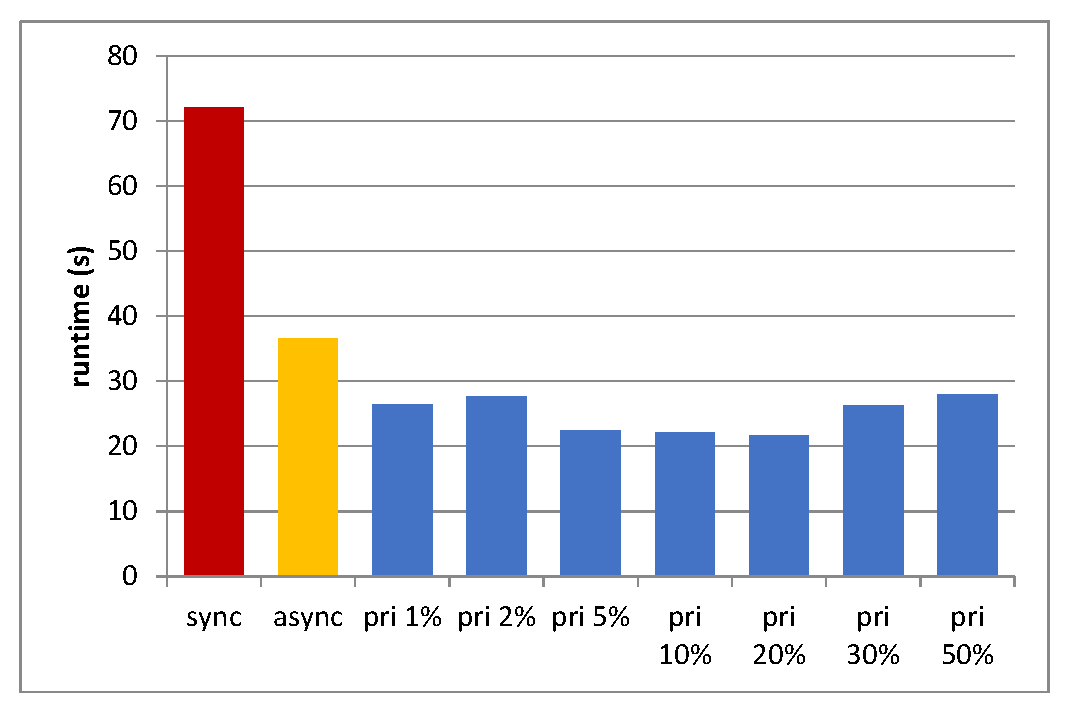
\includegraphics[width=2.8in]{fig/single-granularity}
  \caption{Effect of optimal granularity (shared-memory runtime/PageRank/ClueWeb20M)}
  \label{fig:single-granularity}
  \vspace{-0.2in}
\end{figure}

both shared-memory and distributed
1\% 2\% 5\%, 10\%, 20\% 30\% 50\%, dynamic granularity (can you implement it?)
app: pagerank, CC, LCA, who will come to party
\end{comment}




\section{Related Works}
\label{sec:related}

\Paragraph{Coordination Avoidance} Minimizing coordination, or blocking communication between concurrently executing operations, is key to maximizing scalability, availability, and high performance in database systems. However, uninhibited coordination-free execution can compromise application correctness, or consistency. Coordination and consistency are the most critical issues for system performance and manageability at scale \cite{Bailis:2014:CAD:2735508.2735509}. Hellerstein et al. have set up the foundation \cite{Hellerstein:2010:DIE:1860702.1860704} and have put a lot of efforts to advance this field \cite{Alvaro:2013:CWB:2523616.2523632,Bailis:2014:QEC:2632661.2632792}. Dedalus \cite{Alvaro:2010:DDT:2185923.2185942} is proposed as a declarative foundation for the two signature features of distributed systems: mutable state, and asynchronous processing and communication. CALM (Consistent and Logical Monotonicity) principle \cite{calm} is described for reasoning about distributed system behaviour, which ensures eventual consistency by enforcing a \emph{monotonic} logic. A declarative language called Bloom \cite{Conway:2012:LLD:2391229.2391230} that encourages CALM programming and is well-suited to the inherent characteristics of distribution. Edelweiss \cite{Conway:2014:EAS:2732279.2732285} is a sublanguage of Bloom that provides an Event Log Exchange (ELE) programming model, yet automatically reclaims space without programmer assistance, which can be used to elegantly implement asynchronous communications. Blaze \cite{blaze} ensures consistent outcomes via a more efficient and manageable protocol of asynchronous point-to-point communication between producers and consumers. MacroBase \cite{Bailis:2017:MPA:3035918.3035928} is a fast data system built to explore the fast data principles that suggests asynchronously prioritizing computation on inputs that most affect outputs.


%and have put a lot of efforts to advance this field \cite{Bailis:2012:PDC:2391229.2391251,Bailis:2013:BCC:2463676.2465279,Alvaro:2013:CWB:2523616.2523632,Bailis:2014:QEC:2632661.2632792}
%CRDT \cite{Shapiro:2011:CRD:2050613.2050642} requires every update or merge operation to move forward in the monotonic semilattice. The Potential Dangers of Causal Consistency and an Explicit Solution are identified in \cite{Bailis:2012:PDC:2391229.2391251}. Bolt-on Causal Consistency \cite{Bailis:2013:BCC:2463676.2465279} reformulates the correctness criteria for causal consistency as a more general, declarative specification. In \cite{Alvaro:2013:CWB:2523616.2523632}, Alvaro et al. give a comprehensive discussion of consistency without borders. In \cite{Bailis:2014:QEC:2632661.2632792}, Bailis et al. introduce a consistency model Probabilistically Bounded Staleness (PBS).


%\cite{Alvaro:2010:DDT:2185923.2185942, Alvaro:2010:BAE:1755913.1755937, Conway:2012:LLD:2391229.2391230, Bailis:2012:PDC:2391229.2391251, Bailis:2013:ECT:2460276.2462076, Bailis:2013:BCC:2463676.2465279, Alvaro:2013:CWB:2523616.2523632, Bailis:2014:QEC:2632661.2632792, blaze, Bailis:2014:CAD:2735508.2735509, DBLP:journals/corr/GonzalezBJFHGS15}.

\Paragraph{Asynchronous Computation in Graph Analytics} Asynchronous computation has attracted much attention in the field of graph processing. GraphLab \cite{Low:2012:DGF:2212351.2212354} aims to express asynchronous iterative algorithms with sparse computational dependencies while ensuring data consistency and achieving good parallel performance. Frog \cite{8017445} is a lock-free semi-asynchronous parallel graph processing framework with a graph coloring model. Grace \cite{grace} is a single-machine parallel graph processing platform that allows customization of vertex scheduling and message selection to support asynchronous computation. Giraph++ \cite{Tian:2013:TLV:2732232.2732238} not only allows asynchronous computation while keeping the vertex-centric model but also is able to handle mutation of graphs. GiraphUC \cite{Han:2015:GUB:2777598.2777604} relies on barrierless asynchronous parallel (BAP), which reduces both message staleness and global synchronization. Maiter \cite{maiter} proposes delta-based asynchronous iterative computation model (DAIC) and supports distributed asynchronous graph processing. GunRock \cite{Wang:2016:GHG:2851141.2851145} supports fast asynchronous graph computation in GPUs. Unfortunately, the above graph systems do not support automatic asynchronization.

%Asynchronous MapReduce \cite{asynchronous} proposes to use more local synchronizations to replace global synchronizations to gain performance.

GRAPE \cite{Fan:2017:PSG:3035918.3035942} differs from prior systems in its ability to automatically parallelize existing sequential graph algorithms as a whole. Sequential graph algorithms can be "plugged into" GRAPE with minor changes, and get parallelized. As long as the sequential algorithms are correct, the GRAPE parallelization guarantees to terminate with correct answers under a monotonic condition. However, GRAPE cannot automatically asynchronize a sequential graph algorithm.

%compare with Maiter \cite{maiter}, extended to relational algebral, generalize to aggregation, support to automatically asyncronization, datalog system.

\Paragraph{Asynchronous Computation in Machine Learning} In machine learning, some algorithms with non-serializable lock-free implementations offer significant speedups. Gonzalez et al. \cite{DBLP:journals/corr/GonzalezBJFHGS15} examine the growing gap between efficient machine learning algorithms exploiting asynchrony and fine-grained communication, and commodity distributed dataflow systems (Hadoop and Spark) that are optimized for coarse-grained models. Google DeepMind group recently proposes asynchronous methods for deep reinforcement learning \cite{Mnih:2016:AMD:3045390.3045594}, which surpasses the current state-of-the-art on the Atari domain while training for half the time on a single multi-core CPU instead of a GPU. DimmWitted \cite{Zhang:2014:DSM:2732977.2733001} exposes a range of options for asynchronous data sharing, which outperforms general cluster compute frameworks by orders of magnitude in the context of popular models, including SVMs, logistic regression, Gibbs sampling, and neural networks. HOGWILD! \cite{Niu:2011:HLA:2986459.2986537} is a implementation of stochastic gradient descent (SGD), which places a single copy of the model in the memory of a multi-core server and runs multiple worker processes that simultaneously run gradient steps in parallel. An asynchronous parallel stochastic coordinate descent algorithm is proposed in \cite{Liu:2015:APS:2789272.2789282}, which shows significant speedup in multi-core environment. A burgeoning cottage industry of machine learning researchers has begun to extend asynchronous execution strategies to an increasing number of optimization tasks.

\Paragraph{Datalog Systems}
Besides SociaLite \cite{Lam:2013:SDE:2510649.2511289,Seo:2013:DSD:2556549.2556572} and Myria \cite{Halperin:2014:DMB:2588555.2594530,Wang:2015:AFR:2824032.2824052}, there exist other Datalog systems. DeALS \cite{Shkapsky:2013:GQN:2536274.2536290,7113340} is a deductive database systems relying on Datalog language, supporting optimized execution over diverse platforms including sequential implementations, multi-core machines, and clusters. BigDatalog \cite{Shkapsky:2016:BDA:2882903.2915229} is built on top of Spark \cite{Zaharia:2010:SCC:1863103.1863113} and provides declarative semantics of monotonic aggregate programs. Datalography \cite{7840589} incorporates optimization techniques for efficient distributed evaluation of Datalog queries on Giraph \cite{giraph}. LogicBlox \cite{Aref:2015:DIL:2723372.2742796} is a commercial database system based on LogiQL.


%\Paragraph{Semi-Asynchronous Techniques}
%GraphLab \cite{Low:2012:DGF:2212351.2212354}
%Sequential random permutation, list contraction and tree contraction are highly parallel, dependency tree \cite{Shun:2015:SRP:2722129.2722159}. In such algorithms, instead of waiting for its turn in the sequential order, a given step can run immediately once all previous steps it depends on have been completed. The approach allows for steps to run in parallel while performing the same computations on each step as the sequential algorithm, and consequently returning the same result. \cite{Shun:2015:SRP:2722129.2722159}



%priority scheduling \cite{priori-cidr, Bailis:2017:MPA:3035918.3035928}

%Asynchronous Complex Analytics in a Distributed Dataflow Architecture \cite{DBLP:journals/corr/GonzalezBJFHGS15}





%Reducing the impact of aggregation and improving the parallelism are the fundamental issues in distributed systems. Hellerstein and his group \cite{Hellerstein:2010:DIE:1860702.1860704} have put a lot of research efforts to advance this field \cite{Alvaro:2010:DDT:2185923.2185942, Alvaro:2010:BAE:1755913.1755937, Conway:2012:LLD:2391229.2391230, Bailis:2012:PDC:2391229.2391251, Bailis:2013:ECT:2460276.2462076, Bailis:2013:BCC:2463676.2465279, Alvaro:2013:CWB:2523616.2523632, Bailis:2014:QEC:2632661.2632792, blaze, Bailis:2014:CAD:2735508.2735509, DBLP:journals/corr/GonzalezBJFHGS15}.

%\cite{Ameloot:2014:DNR:2694413.2694415}






\section{Conclusions}
\label{sec:conclusion}

We have presented A3, Automatic Asynchronous Aggregation. We clearly define the conditions for asynchronous aggregation and propose to prioritize the aggregate computations that most affect result. We also propose a technique to allow automatic asynchronization. We further design and implement a Datalog system, A3Log, to support automatic asynchronous computation of the user's program. A3Log provides both shared-memory runtime and distributed runtime. Our results show that A3Log outperforms the state-of-the-art systems for various applications. Asynchronous execution is shown to achieve up to two-orders-of-magnitude speedup over synchronous execution.

\pagebreak





\begin{comment}
\section{Delta Monotonic Aggregates}

\subsection{Semantics}

The delta monotonic aggregate operation $g$ is used in recursive aggregations. It aggregates a set of values to $\Delta v$ and further monotonically aggregates $\Delta v$ to a maintained value $v$. We provide the formal definition of \emph{delta monotonic aggregate} operation as follows.

\begin{definition}
\label{def:daggr}
Given any normal aggregate operator $\oplus$, the delta monotonic aggregate operation $g$ defined over $\oplus$ aggregates a number of values $v_1,\ldots,v_n$ to $\Delta v$ and monotonically update the maintained $v$ in a two-step manner.
\begin{equation}\label{eq:daggr}
\begin{aligned}
g(v_1,\ldots,v_n): \quad &\Delta v=v_1\oplus v_2\oplus \ldots\oplus v_n;\\
                    &v=v\oplus \Delta v.
\end{aligned}
\end{equation}
The initial $v$ is set to the identity element\footnote{The identity element is a special type of element of a set with respect to a binary operation on that set, which leaves other elements unchanged when combined with them.} with respect to the specific aggregation function.
\end{definition}

Suppose the normal aggregate operator $\oplus$ could be \texttt{max}, \texttt{min}, \texttt{sum}, \texttt{count}, etc. We have correspondingly define a series of delta monotonic aggregate operators \texttt{dmax}, \texttt{dmin}, \texttt{dsum}, \texttt{dcount}, etc. Users also have the option to define their own delta monotonic aggregators based on Definition \ref{def:daggr}.

The Datalog program with a recursive and delta monotonic aggregate is typically written with the following form. It is repeatedly evaluated until convergence.
\begin{lstlisting}
  P($x_1,\ldots,x_m,g[\Delta v]$) $\leftarrow$ P($x_1,\ldots,x_m,\Delta v'$),
                    Q$_1$($x_1,\ldots,x_m,w_1$),
                    ...
                    Q$_k$($x_1,\ldots,x_m,w_k$),
                    $\Delta v=f(\Delta v',w_1,\ldots,w_k)$,
                    [termination condition].
\end{lstlisting}

\texttt{P} is the recursive defined part. \texttt{Q}$_i$ ($1\leq i\leq k$) is the other facts that support the query. $x_1,\ldots,x_m$ are the \emph{group-by arguments} (which could be zero). $w_1,\ldots,w_k$ are the values retrieved from facts Q$_1,\ldots,$Q$_k$. $f$ is a user-defined function applied on $\Delta v'$. $g$ is the \emph{delta monotonic aggregate operator}, and $[\Delta v]$ is a set of \emph{delta aggregate variables}.

%\cite{Zhao:2017:AGP:3035918.3035943}
\Paragraph{Termination Condition} In traditional Datalog, the recursive query terminates when no new facts is found. This follows the fixpoint theory. However, as we extend Datalog to support aggregations, it is possible that some new facts are found continuously even though their \emph{contribution}\footnote{The new facts are aggregated to be values which can be identified as contributions to final result.} to the final result is less and less. Therefore, we should correspondingly extend Datalog language to help users specify how to terminate based on the aggregated values, i.e., whether the current contribution is enough for convergence.

The \textbf{termination condition} defines how the recursive query ends. We allow users to define their own termination condition in the [] part.
\begin{enumerate}
  \item To be as much general as possible, users can use an aggregation that combines the global information to make the decision. For example, $[sum(v)>0.999]$ in PageRank, $[sum(\Delta v)=0]$ in SSSP.
  \item We allow users to use \texttt{any} and \texttt{all} as shortcut to check termination condition. For example, $[any \Delta v<0]$, $[all v>1]$. Note that, this can also be realized equally by using aggregation ($[max(Delta v)<0]$, $[min(v)>1]$).
  \item The recursive query sometimes can be decomposed into multiple individual record-level queries. This is common in graph queries where each query can be decomposed into multiple node-level queries. As stated in \cite{Low:2012:DGF:2212351.2212354}, the recursive query with multiple node-level queries can be terminated individually rather than terminated synchronously. So we also allow users to specify individually termination check. For example, $[\Delta v < 0.0001]$ in PageRank indicates that if the node ranking score change is less than 0.0001, the node is considered as converged and will not involve in next iteration.
  \item If no termination condition is specified, the recursive query terminates when there is no new facts found.
  \item If multiple termination conditions are defined, it terminates when any of termination conditions is met. Multiple termination conditions can be defined as follows, $[termination condition 1][termination condition 2][\ldots]$.
  \item In the synchronous execution case, the termination condition check is launched after every iteration. In the asynchronous execution case, the termination condition check is launched every other a certain time interval. Users can specify the time interval $T$ in millisecond unit after [], e.g., [termination condition](10000).
\end{enumerate}

\Paragraph{Evaluation} During evaluation, the rule body is \textbf{only} allowed to use the aggregated delta values $\Delta v$ retrieved in previous recursion \textbf{rather than} using the updated maintained variable $v$. $v$ is not exposed to users but it stores the final result. While in non-recursive rules, the aggregation result $v$ is used for evaluation. In other words, each key is associated with two variables, i.e., not only $v$ but also $\Delta v$ that depicts the monotonically increase/decreased value. The evaluation terminates when the aggregated delta value $[\Delta v]$ means nothing, i.e., $[\Delta v]\oplus v=v$.

To generalize the recursively defined rule, more than one rules could be involved in a recursion.

\begin{lstlisting}
  R$_1$($x_1,\ldots,x_m$,X$_1$) $\leftarrow$ P($x_1,\ldots,x_m,v$),
  ...
  R$_j$($x_1,\ldots,x_m$,X$_j$) $\leftarrow$ R$_{j-1}$($x_1,\ldots,x_m$,X$_{j-1}$),
  P($x_1,\ldots,x_m,g[\Delta v]$) $\leftarrow$ R$_j$($x_1,\ldots,x_m$,X$_j$).
\end{lstlisting}

We omit the other facts and only leave the rules related to delta monotonic aggregation for describing each rule. Regarding the rule that is not recursively defined, fact \texttt{P} uses $v$ instead of $\Delta v$ for evaluation as shown in the first rule. Semi-naive evaluation will be used to evaluate the rules. When evaluating the last rule, the newly discovered facts $\Delta$\texttt{X}$_j$ is used to identify delta values $[\Delta v]$ which will be aggregated and used to update $v$.

\Paragraph{Equivalence to Semi-Naive Evaluation} When evaluating the recursive datalog program with this semantics, new fact is generated if and only if $v$ is updated, and it will be used in next recursion. Otherwise, no new fact is generated, and it will terminate the recursion on this fact. Let us rethink the semi-naive evaluation of the Datalog program with recursive aggregations. The semi-naive evaluation operates on newly discovered facts. It is an optimization critical to the efficient execution of recursive Datalog rules. While with aggregation functions, the incremental sets can be transformed to delta values. The delta values implicitly indicate the aggregated values obtained from the incremental sets. Therefore, rather than evaluating on incremental sets, we can evaluate on delta values to achieve the same cost-effective goal. The recursive Datalog program with our delta monotonic aggregates actually simulates the traditional semi-naive evaluation while with much less space cost, since we already transform the relatively large set of data to only two values $v$ and $\Delta v$.



\subsection{Benefits}

\Paragraph{Fixpoint Guarantee} When viewed as a sequence, the maintained variable $v$ is updated monotonically. We have shown the equivalence between delta monotonic aggregate and semi-naive evaluation. Similar to \cite{Lam:2013:SDE:2510649.2511289}, we have the following theorem \cite{fixpoint}.


\begin{theorem}
Given a set of recursive rules written with delta aggregate function $g$ in a Datalog program, let $f$ represent the rest of rules. If the aggregation $g$ defines a partial order $\preccurlyeq$ where $g(X)\preccurlyeq g(X\cup Y)$ for any $Y$ in a finite domain, and $f$ is monotone with respect to the partial order $\preccurlyeq$, then there exists a unique greatest fixed point.
\end{theorem}
\begin{proof}
\end{proof}

Following \cite{Lam:2013:SDE:2510649.2511289}, we have the following theorem.
\begin{theorem}
\label{the:delta}
The recursive datalog programs with delta monotonic aggregate will yield the same greatest fixpoint as that with normal aggregate, as long as $g$ is commutative, associative, and $g\circ g(X)=g(X)$.
\end{theorem}
\begin{proof}
Suppose an arbitrary aggregation $g$ and the recursive datalog program with $g$ starts from $V_0$ and converges to a fixpoint $V_i$. That is,
\begin{equation}
V_0\preccurlyeq V_1=g(f(V_0))\preccurlyeq\ldots\preccurlyeq V_i=g(f(V_{i-1}))=g(f(V_{i}))
\end{equation}
Delta monotonic aggregate remembers the previous aggregation result $V_{i-1}$ and only performs operations on $\Delta V_i$, i.e., $V_{i}=g(V_{i-1}\cup \Delta V_i)$. So we have
\begin{equation}\label{eq:delta}
\begin{aligned}
V_{i}&=g(V_{i-1}\cup \Delta V_i)\\
        &=g(V_{i-1}\cup f(\Delta V_{i-1}))\\
       &=g(g(V_{i-2}\cup f(\Delta V_{i-2}))\cup f(\Delta V_{i-1}))\\
       &=\ldots\\
       &=g(f(\Delta V_0)\cup f(\Delta V_1)\cup\ldots\cup f(\Delta V_{i-1}))\\
       &=g(f(\Delta V_0\cup\Delta V_1\cup\ldots\cup\Delta V_{i-1}))\\
       &=g(f(V_{i-1}))
\end{aligned}
\end{equation}
Note that, the fourth line is true since $g\circ g(X)=g(X)$.
\end{proof}


\Paragraph{Cost Effective} The recursive aggregation with delta monotonic aggregators is somehow like semi-naive evaluation. The delta monotonic aggregate operates on incremental values, while semi-naive evaluation operates on incremental set. Both of them can save a lot of computation cost. Just like semi-naive evaluation, delta monotonic aggregate can avoid a lot computations if $\Delta v$ is zero or small enough, which is \textbf{computation-effective}. Furthermore, the evaluation with delta aggregate is much more space \textbf{cost-effective}. Instead of maintaining a set of incremental sets of data, we only need to maintain two values $v$ and $\Delta v$ for each item.

\Paragraph{Possibility of Asynchronous Evaluation}




\subsection{Scheduling of Aggregation Operations}
\label{sec:order}

look at this post to see how they motivate prioritized computation. https://blog.acolyer.org/2017/01/19/prioritizing-attention-in-fast-data-principles-and-promise/
Prioritizing attention in fast data: principles and promise CIDR 2017

given an expected fixpoint, pick the aggregation operations that contribute more on approaching the fixpoint. with proof.

\begin{theorem}
If the $g\circ f$ operations with larger aggregated $\Delta V$ (based on the partial order induced by $g\circ f$) are scheduled first, we will need less or equal to the number of operations needed by synchronous aggregation.
\end{theorem}
\begin{proof}
They are approaching to the fixpoint at a relatively quick pace.
\end{proof}
\end{comment}



\bibliographystyle{ACM-Reference-Format}
% argument is your BibTeX string definitions and bibliography database(s)
\bibliography{./new}

\appendix

\section{Proofs}

\subsection{Proof of Theorem \ref{th:monotone}}
\label{sec:app:proof:monotone}

\begin{proof}
Since $X^{k-1}\subseteq f\circ g(X^{k-1})=X^k$, we have $X^{k}=X^{k-1}\cup\Delta X^{k}$ where $\Delta X^{k}=X^{k}\setminus X^{k-1}$. Let $x^{k}$ denote the result of normal recursive program and $\bar{x}^{k}$ denote the result of accumulated recursive program after $k$ recursions. Then we have
%We use mathematical induction to show that $x^{k}=\bar{x}^{k}$. Suppose $x^{0}=\Delta x^0$, in the basic step we have $\bar{x}^{1}=g\circ f(\Delta x^0)=g\circ f(x^0)=x^1$. In the deductive step, assuming $x^{k}=\bar{x}^{k}$ for all $k\leq i$, then we have
\begin{align}\label{eq:monotoneproof}
  x^{k}&=g(X^{k})=g(X^{k-1}\cup \Delta X^{k}) \tag{1}\\
          &=\ldots \tag{2}\\
          &=g(\Delta X^{0}\cup\ldots\cup \Delta X^{k-1}\cup \Delta X^{k}) \tag{3}\\
          &=g(g(\Delta X^{0})\cup\ldots\cup g(\Delta X^{k-1})\cup g(\Delta X^{k})) \tag{4}\\
          &=g(\Delta x^{0},\ldots,\Delta x^{k-1},\Delta x^{k})=\bar{x}^{k}. \tag{5}
\end{align}
Line (1)-(3) are true because of the monotonicity. Due to the accumulativity and commutativity, we have $g(X_1\cup X_2)=g(g(X_1)\cup X_2)=g(X_2\cup g(X_1))=g(g(X_1)\cup g(X_2))$, from which Line (4) is true. Line (5) is true because of the definition of accumulated recursive program.
\end{proof}


\subsection{Proof of Theorem \ref{th:async}}
\label{sec:app:proof:async}

\begin{proof}
Let $\Delta X_{1}^{k}$ and $\Delta X_{2}^{k}$ denote two disjoint subsets of $\Delta X^{k}$, where $\Delta X^{k}$ is the intermediate result of the $k$th recursion in accumulated recursive program. If the aggregation is performed across any two recursions (which can be easily extended to any multiple recursions), i.e., $g(\Delta X_{1}^{k}\cup \Delta X_{1}^{l})$ where $k\neq l$, and the result is the same as that in synchronous aggregation, the theorem is proved.

%The program can be executed asynchronously means that for any combination of any subset of $\Delta V_j$ can be aggregated together without considering the aggregation order of $\Delta V_0\rightarrow\Delta V_1\rightarrow\ldots\rightarrow\Delta V_i$.

%Suppose $\Delta V_{ka}$ is a subset of $\Delta V_k$ (i.e., $\Delta V_{ka}\cup\Delta V_{kb}=\Delta V_k$) and $\Delta V_{jb}$ is a subset of $\Delta V_j$ (i.e., $\Delta V_{ja}\cup\Delta V_{jb}=\Delta V_j$). If we can prove that $\Delta V_{ka}$ and $\Delta V_{jb}$ can be aggregated without the constraint that $\Delta V_{ka}$ and $\Delta V_{kb}$ have to be aggregated first, the theorem is proved.

{\small
\begin{align}\label{eq:asyncproof}
    &g(\Delta X^0\cup\ldots g(\Delta X_{1}^{k+1}\cup\Delta X_{1}^{l+1})\cup\Delta X_{2}^{k+1}\cup\Delta X_{2}^{l+1}\ldots\cup\Delta X^n) \tag{1}\\
    =&g(\Delta X^0\cup\ldots g(\Delta X_{1}^{k+1}\cup\Delta X_{1}^{l+1})\cup g(\Delta X_{2}^{k+1}\cup\Delta X_{2}^{l+1})\ldots\cup\Delta X^n) \tag{2}\\
    =&g(\ldots g(f\circ g(\Delta X_{1}^{k})\cup f\circ g(\Delta X_{1}^{l}))\cup g(f\circ g(\Delta X_{2}^{k})\cup f\circ g(\Delta X_{2}^{l}))\ldots) \tag{3}\\
    =&g(\ldots g\circ f(\Delta X_{1}^{k})\cup g\circ f(\Delta X_{1}^{l})\cup g\circ f(\Delta X_{2}^{k})\cup g\circ f(\Delta X_{2}^{l})\ldots) \tag{4}\\
    =&g(\ldots g\circ f(\Delta X_{1}^{k}\cup \Delta X_{2}^{k})\cup g\circ f(\Delta X_{1}^{l}\cup\Delta X_{2}^{l})\ldots) \tag{5}\\
    =&g(\ldots f\circ g(\Delta X_{1}^{k}\cup \Delta X_{2}^{k})\cup f\circ g(\Delta X_{1}^{l}\cup\Delta X_{2}^{l})\ldots) \tag{6}\\
    =&g(\Delta X^0\cup\ldots\cup\Delta X^{k+1}\cup \Delta X^{l+1}\cup\ldots\cup\Delta X^n) \tag{7}
\end{align}
}
Line (2) is true because of the accumulative and commutative properties of $g$ operation which is required by accumulated recursive program (i.e., $g(X\cup Y)=g(X\cup g(Y))$). Line (3) is true because of Equation (\ref{eq:accumasync}). Line (4) is true because $g\circ f\circ g(X)=g\circ f(X)$. Line (5) is true because $g(g(X_1)\cup g(X_2))=g(X_1\cup X_2)$ (from accumulative and commutative properties) and the distributive property of $f$ operation. Line (6) is true because $g\circ f(X)=g\circ f\circ g(X)$ and $g(g(X_1)\cup g(X_2))=g(X_1\cup X_2)$. Line (7) is the result of synchronous recursion. Therefore, by asynchronous aggregation, the accumulated recursive program will yield to the same result as synchronous aggregation.
\end{proof}

\subsection{Proof of Theorem \ref{th:convert}}
\label{sec:app:proof:convert}

\begin{proof}
Let $g(X^0)=x^0$, then we have
\begin{align}\label{eq:accumproof}
     &(g\circ f)^{n}(x^0)=(g\circ f)^{n}\circ g(X^0) \tag{1}\\
    =&g\circ f\circ g\circ\ldots\circ g\circ f\circ g'(X^0\cup y) \tag{2}\\
    =&g\circ f\circ g\circ\ldots\circ g'\Big((f\circ g')(X^0\cup y)\cup y\Big) \tag{3}\\
    =&g\circ f\circ g\circ\ldots\circ g'\Big((f\circ g')(X^0)\cup f(y)\cup y\Big) \tag{4}\\
    =&... \tag{5}\\
    =&g'\Big((f\circ g')^{n}(X^0)\cup f^n(y)\cup \ldots\cup f(y)\cup y\Big) \tag{6}\\
    =&g'\Big(f^{n}(y),\ldots,f(y),y\Big) \tag{7}
\end{align}
Line (2) is true because $g(X)=g'(X\cup y)$. Line (3) is true because $g'(X_1\cup X_2)=g'\Big(g'(X_1)\cup g'(X_2)\Big)$. Line (4) is true because the distributive property of $f()$. Since \textbf{0} is the identity of $g'()$ function, i.e., $g'(X\cup \textbf{0})=g'(X)$, Line (6) is true when the recursion performs infinite times, i.e., $n\rightarrow\infty$. Line (7) is in the result format of accumulated recursive program, which implies that the normal recursive program is converted to the accumulated recursive program.
\end{proof}



\section{Datalog Examples}
\label{sec:app:example}

\begin{verbatim}
  Program 3. Connected Conponents
\end{verbatim}\vspace{-0.1in}\small
\begin{lstlisting}
  r1. cc(X,X)$\leftarrow$ edge(X,_).
  r2. cc(Y,min[$v$])$\leftarrow$ cc(X,$v$),edge(X,Y),
                     cc(Y,$v$).
\end{lstlisting}
\normalsize

Program 3 computes the connected components in a graph. Each vertex starts as its own connected component with its identifier. For all combinations of facts that satisfy the recursive bodies, the aggregate function \texttt{min} keeps and propagates only the current minimal component ID $v$ for each vertex \texttt{Y}.

\begin{verbatim}
  Program 4. Computing Paths in a DAG
\end{verbatim}\vspace{-0.1in}\small
\begin{lstlisting}
  r1. cpaths(X,Y,$c$) $\leftarrow$ edge(X,Y), $c=1$.
  r2. cpaths(X,Y,count[$c$]) $\leftarrow$ cpaths(X,Z,$c$),
                              edges(Z,Y),
                              cpaths(X,Y,$c$).
\end{lstlisting}
\normalsize

Program 4 counts the paths between pairs of vertices in an acyclic graph. \texttt{r1} counts each edge as one path between its vertices. In \texttt{r2}, any \texttt{edge(Z,Y)} that extends from a computed path count \texttt{cpath(X,Z,$c$)} establishes $c$ distinct paths from \texttt{X} to \texttt{Y} through \texttt{Z}.


\begin{verbatim}
  Program 5. Max Probability Path
\end{verbatim}\vspace{-0.1in}\small
\begin{lstlisting}
  r1. reach(X,Y,$P$) $\leftarrow$ net(X,Y,$P$).
  r2. reach(X,Y,max[$P$]) $\leftarrow$ reach(X,Z,$P1$),
                           reach(Z,Y,$P2$),
                           $P=P1*P2$,
                           reach(X,Y,$P$).
\end{lstlisting}
\normalsize

Program 5 \cite{7113340} computes the max probability path between two nodes in a network. The \texttt{net} predicate denotes the probability \texttt{P} of reaching \texttt{Y} from \texttt{X}.

\begin{verbatim}
  Program 6. Least Common Ancestor
\end{verbatim}\small
\begin{lstlisting}
  r1. ancestor(Y,X,1) $\leftarrow$ cite(Y,X), X<seed.
  r2. ancestor(Z,X,min[$d$]) $\leftarrow$ ancestor(Z,Y,$d'$),
                              cite(Y,X),$d=d'+1$,
                              ancestor(Z,X,$d$).
  r3. LCA(p1,p2,min[max(  $\leftarrow$ ancestor(p1,X,d1),
        d1,d2)],year,X)      ancestor(p2,X,d2),
                             Paper(X,year),
                             p1<p2.
\end{lstlisting}
\normalsize

Program 6 \cite{Wang:2015:AFR:2824032.2824052} computes the least common ancestor (LCA) for pairs of publications in a citations graph. An ancestor a of a paper \texttt{Z} is any paper that is transitively cited by \texttt{Z}, and the LCA a of two papers \texttt{X} and \texttt{Y} is the least ancestor of both \texttt{X} and \texttt{Y}.

\begin{verbatim}
  Program 7. What is the cost of each part
\end{verbatim}\vspace{-0.1in}\small
\begin{lstlisting}
  r1. cost(Part,$\mathcal{C}$) $\leftarrow$ basic(Part,cost).
  r2. cost(Part,sum[$\mathcal{C}$]) $\leftarrow$ assb(Part,Sub,$n$),
                           cost(Sub,$c$),
                           $\mathcal{C}=c*n$,
                           cost(Part,$\mathcal{C}$).
\end{lstlisting}
\normalsize

Program 7 \cite{7113340} is for computing the cost of a part from the cost of its subparts. The \texttt{assb} predicate denotes each part��s required subparts and number required, and basic denotes the part��s cost.

\begin{verbatim}
  Program 8. Viterbi Algorithm
\end{verbatim}\vspace{-0.1in}\small
\begin{lstlisting}
  r1. calcV(0,X,max($L$)) $\leftarrow$ s(0,EX),p(X,EX,$L1$),
                            pi(X,$L2$),$L=L1*L2$.
  r2. calcV($T$,Y,max[$L$]) $\leftarrow$ s($T$,EY),p(Y,EY,$L1$),
                            $T1=T-1$,t(X,Y,$L2$),
                            calcV($T1$,X,$L3$),
                            $L=L1*L2*L3$.
\end{lstlisting}
\normalsize

Program 8 \cite{7113340} is the Viterbi algorithm for hidden Markov models. \texttt{t} denotes the transition probability \texttt{L2} from state \texttt{X} to \texttt{Y}; \texttt{s} denotes the observed sequence of length \texttt{L+1}; \texttt{p} denotes the likelihood \texttt{L1} that state \texttt{X (Y)} emitted \texttt{EX (EY)}. \texttt{r1} finds the most likely initial observation for each \texttt{X}. \texttt{r2} finds the most likely transition for observation \texttt{T} for each \texttt{Y}.

\begin{verbatim}
  Program 9. Who will come to the party?
\end{verbatim}\small
\begin{lstlisting}
  r1. coming(X) $\leftarrow$ sure(X).
  r2. coming(X) $\leftarrow$ cntComing(X,$N$), $N\geq 3$.
  r3. cntComing(Y,count[*]) $\leftarrow$ friend(Y,X),
                              coming(X).
\end{lstlisting}
\normalsize

In this program, some people will come to the party for sure, whereas others only join when at least three of their friends are coming. Program 9 \cite{7113340} describes the retrieving process. With \texttt{cntComing}, each person watches the number of their friends that are coming grow, and once that number reaches three, the person will then come to the party too.

\begin{verbatim}
  Program 10. Galaxy Evolution
\end{verbatim}\small
\begin{lstlisting}
  r1. galaxies(1,gid) $\leftarrow$ galaxies_seed(gid).
  r2. galaxies(t+1,gid2) $\leftarrow$ galaxies(t,gid1),
                            edges(t,gid1,gid2,c),
                            c$\geq$threshold.
  r3. edges(t,gid1,gid2, $\leftarrow$ galaxies(t,gid1),
        count[*])           particles(pid,gid1,t),
                            particles(pid,gid2,t+1).
\end{lstlisting}
\normalsize

Program 10 \cite{Wang:2015:AFR:2824032.2824052} computes the history of a set of galaxies in an astrophysical simulation. The history of a galaxy is the set of past galaxies that merged over time to form the galaxy of interest at present day. The predicate \texttt{Particles(pid,gid,t)} holds the simulation output as a set of particles, where \texttt{pid} is a unique particle identifier, and \texttt{gid} is the identifier of the galaxy that the particle belongs to at time \texttt{t}. The \texttt{gid} values are unique only within their timesteps \texttt{t}, but a particle retains the same \texttt{pid} throughout the simulation.


\begin{verbatim}
  Program 11. Belief Propagation
\end{verbatim}\small
\begin{lstlisting}
  r1. G(v,0) $\leftarrow$ E(v,_,_).
  r2. B(v,c,b) $\leftarrow$ E(v,c,b).
  r3. G(t,i) $\leftarrow$ G(s,i-1),A(s,t,w),$\neg$G(t,_).
  r4. B(t,c2,sum[b']) $\leftarrow$ G(t,i),A(s,t,w),
                         B(s,c1,b),
                         G(s,i-1),H(c1,c2,h),
                         b'=w*b*h,
                         [sum$[\Delta b']<T$];
\end{lstlisting}
\normalsize

Belief Propagation \cite{910572} is a message-passing algorithm for performing inference on graphical models, such as Bayesian networks and Markov random fields. In Program 11, \texttt{B} is the to-be-returned beliefs, \texttt{G} maintains the geodesic numbers, \texttt{A} is an input weighted network with initial beliefs \texttt{E}, and \texttt{H} is the coupling scores. \texttt{r3} and \texttt{r4} should be repeated evaluated where the geodesic number \texttt{i} is increasing, and stops when no more facts inserted into \texttt{G}. Note that, the shown Datalog program describes a single-pass belief propagation process since it does not allow loopy propagation (by $\neg$\texttt{G(t,\_)} in \texttt{r3}) \cite{Gatterbauer:2015:LSB:2735479.2735490}.

\begin{verbatim}
  Program 12. SimRank
\end{verbatim}\small
\begin{lstlisting}
  r1. D(X,count[*]) $\leftarrow$ E(X,Y).
  r2. S(X,Y,1) $\leftarrow$ E(X,Y).
  r3. S(X,Y,sum[s']) $\leftarrow$ S(X',Y',s),E(X,X'),E(Y,Y'),
                        D(X,d1),D(Y,d2),X$\neq$Y,
                        s'=$\frac{C}{d1*d2}$*s,
                        [sum$[\Delta s']<T$].
\end{lstlisting}
\normalsize

SimRank algorithm \cite{Jeh:2002:SMS:775047.775126} is an algorithm to evaluate the similarities between node pairs in a graph. In Program 12, \texttt{S} maintains the similarities between node pairs, \texttt{E} is the edge data, \texttt{D} maintains the out degree information. The algorithm terminates when the sum of differences between two recursions is small enough.

\begin{verbatim}
  Program 13. Jacobi Method
\end{verbatim}\small
\begin{lstlisting}
  r1. X(i,x) $\leftarrow$ X(i,1).
  r2. C(i,c) $\leftarrow$ A(i,i,$a_{ii}$),B(i,$b_i$),
                c=$\frac{b_i}{a_{ii}}$.
  r3. X(i,sum[x']+c) $\leftarrow$ X(j,x),A(i,j,$a_{ij}$),
                        C(i,c),A(i,i,$a_{ii}$),i$\neq$j,
                        x'=$-\frac{a_{ij}}{a_{ii}}$*x,
                        [sum$[\Delta x']<T$].
\end{lstlisting}
\normalsize

In numerical linear algebra, the Jacobi method is a famous iterative algorithm for solving linear equations of the form $A\cdot X=b$, where $A$ is a matrix with each entry $a_{ij}$, and b is a vector with each entry $b_i$. In Program 13, \texttt{X} is the solution vector, \texttt{A} is the matrix, \texttt{B} is the vector, \texttt{C} is a vector maintaining the entry-specific constant $\frac{b_i}{a_{ii}}$. A sufficient (but not necessary) condition for the method to converge is that the matrix \texttt{A} is strictly or irreducibly diagonally dominant, i.e., $|a_{ii}>\sum_{j\neq i}{|a_{ij}|}|$, which implies the convertable condition, so Jacobi Method can be converted and executed asynchronously.


\section{More Experiments}
\label{sec:app:expr}

\subsection{Scaling Performance}
\label{sec:expr:scale}

\begin{comment}
\begin{figure}[t]
%\vspace{-0.1in}
	\centerline{
	\subfloat[Shared-memory]{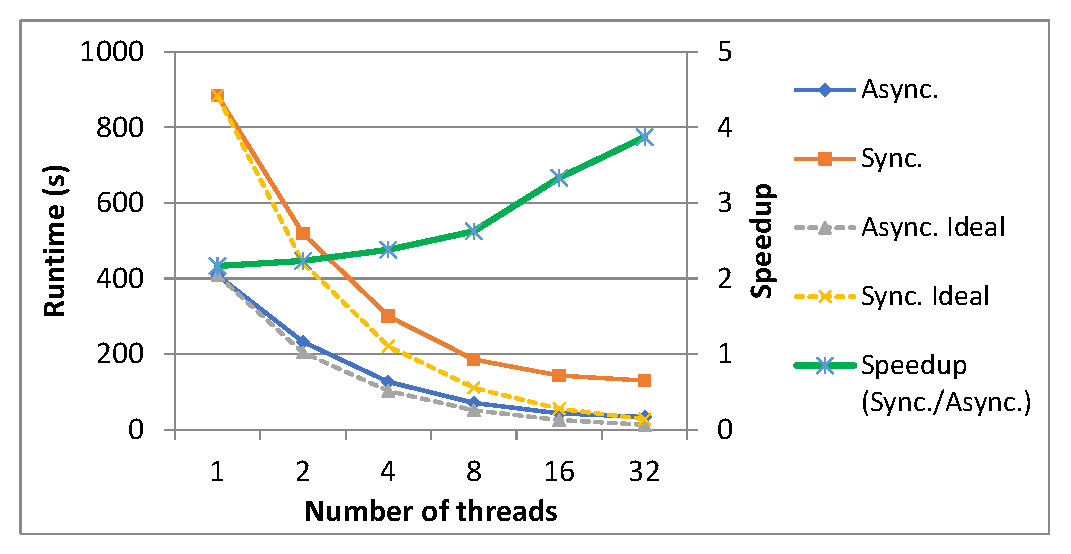
\includegraphics[width=1.8in]{fig/single-scalability}
    \label{fig:single-scalability}
    \vspace{-0.05in}}
    \hspace{-5mm}
    \subfloat[Distributed]{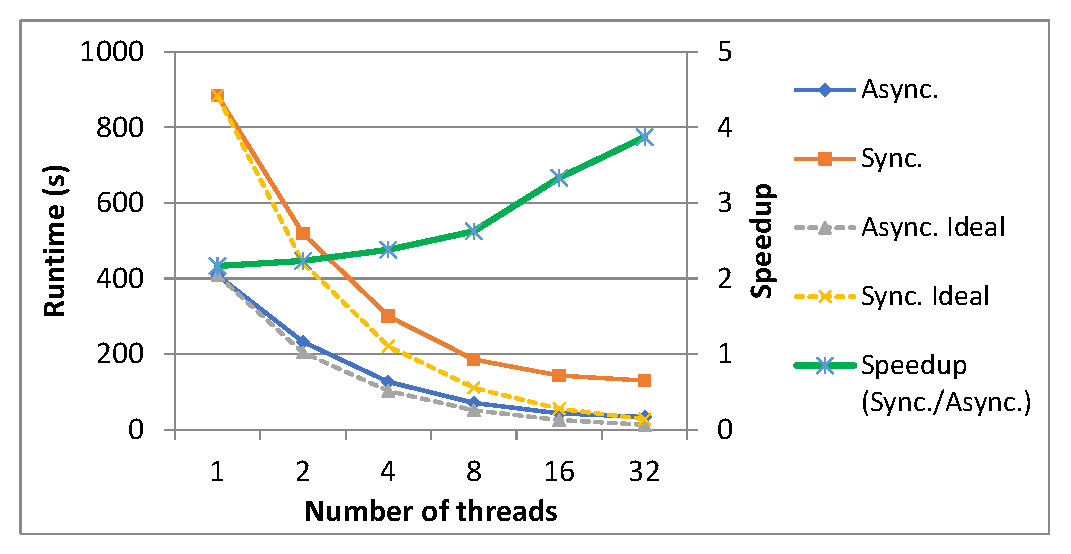
\includegraphics[width=1.8in]{fig/single-scalability}
    \label{fig:distributed-scalability}
    \vspace{-0.05in}}
    }
    %\vspace{-0.05in}
	\caption{The scaling performance (PageRank)}
	\label{fig:scalability}
%\vspace{-0.2in}
\end{figure}
\end{comment}

\begin{figure}[!t]
    \centering
  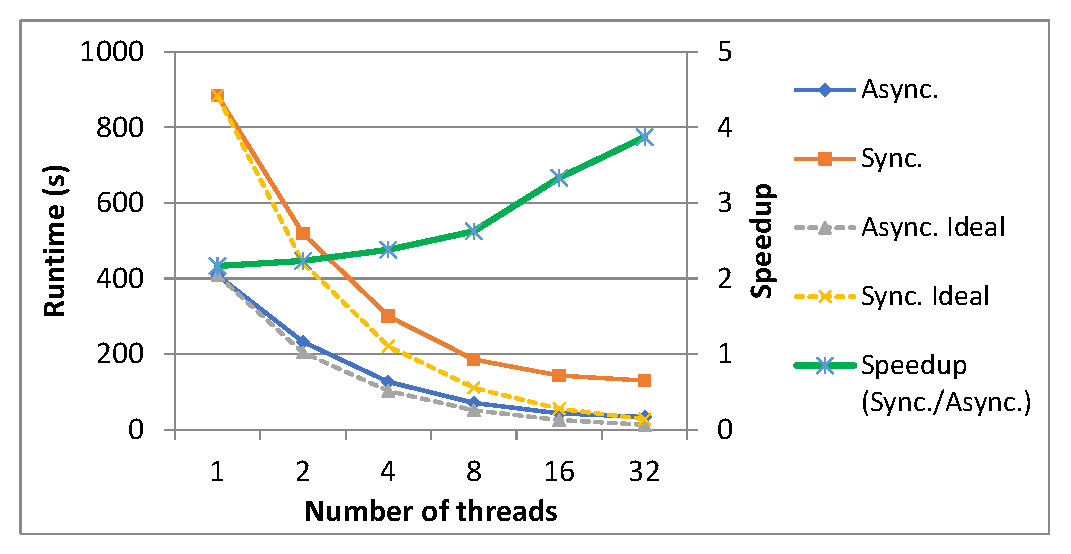
\includegraphics[width=2.8in]{fig/single-scalability}
  \vspace{-0.1in}
  \caption{Scaling performance (many-core)}
  \label{fig:single-scalability}
\end{figure}

\begin{figure}[!t]
    \centering
  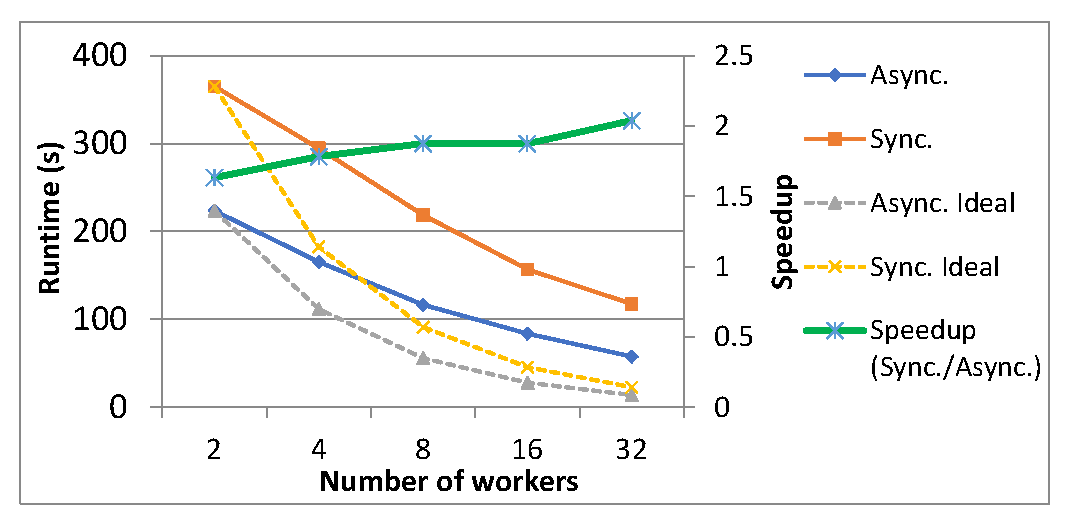
\includegraphics[width=2.8in]{fig/dist-scalability}
  \vspace{-0.1in}
  \caption{Scaling performance (distributed)}
  \label{fig:dist-scalability}
\end{figure}


Due to coordination avoidance, asynchronous aggregation is expected to achieve better scaling performance. We evaluate the scaling performance of A3Log's share-memory runtime on an r3.8xlarge EC2 instance. We perform PageRank computation with the synchronous and asynchronous versions (without scheduling) of A3Log and vary the number of threads from 1 to 32. The runtime results are shown in Fig. \ref{fig:single-scalability}. We also draw the ideal scaling performance curve based on the runtime result of 1 thread. The asynchronous A3Log's scaling performance curve is closer to its ideal curve, while the synchronous A3Log exhibits larger difference to its ideal curve when running on more threads. Asynchronous execution also shows higher speedup over synchronous execution when running on more threads.

We also evaluate the scaling performance of A3Log's distributed runtime on a cluster with a number of c4.large EC2 instances, each with 2 vCPUs and 3.75GB memory. We perform PageRank computation with the synchronous and asynchronous executions (without scheduling) and vary the number of workers from 1 to 32. The runtime results are shown in Fig. \ref{fig:dist-scalability}. We also draw the ideal scaling performance curve based on the runtime result of 2-workers. Similar to the results on shared-memory runtime, asynchronous execution also shows better scaling performance. Higher speedup over synchronous execution is achieved when running on larger size cluster.


\subsection{Effectiveness of Aggregate Operations}
\label{sec:expr:aggregations}

\begin{figure}[!t]
%\vspace{-0.1in}
	\centerline{
	\subfloat[RoadCA]{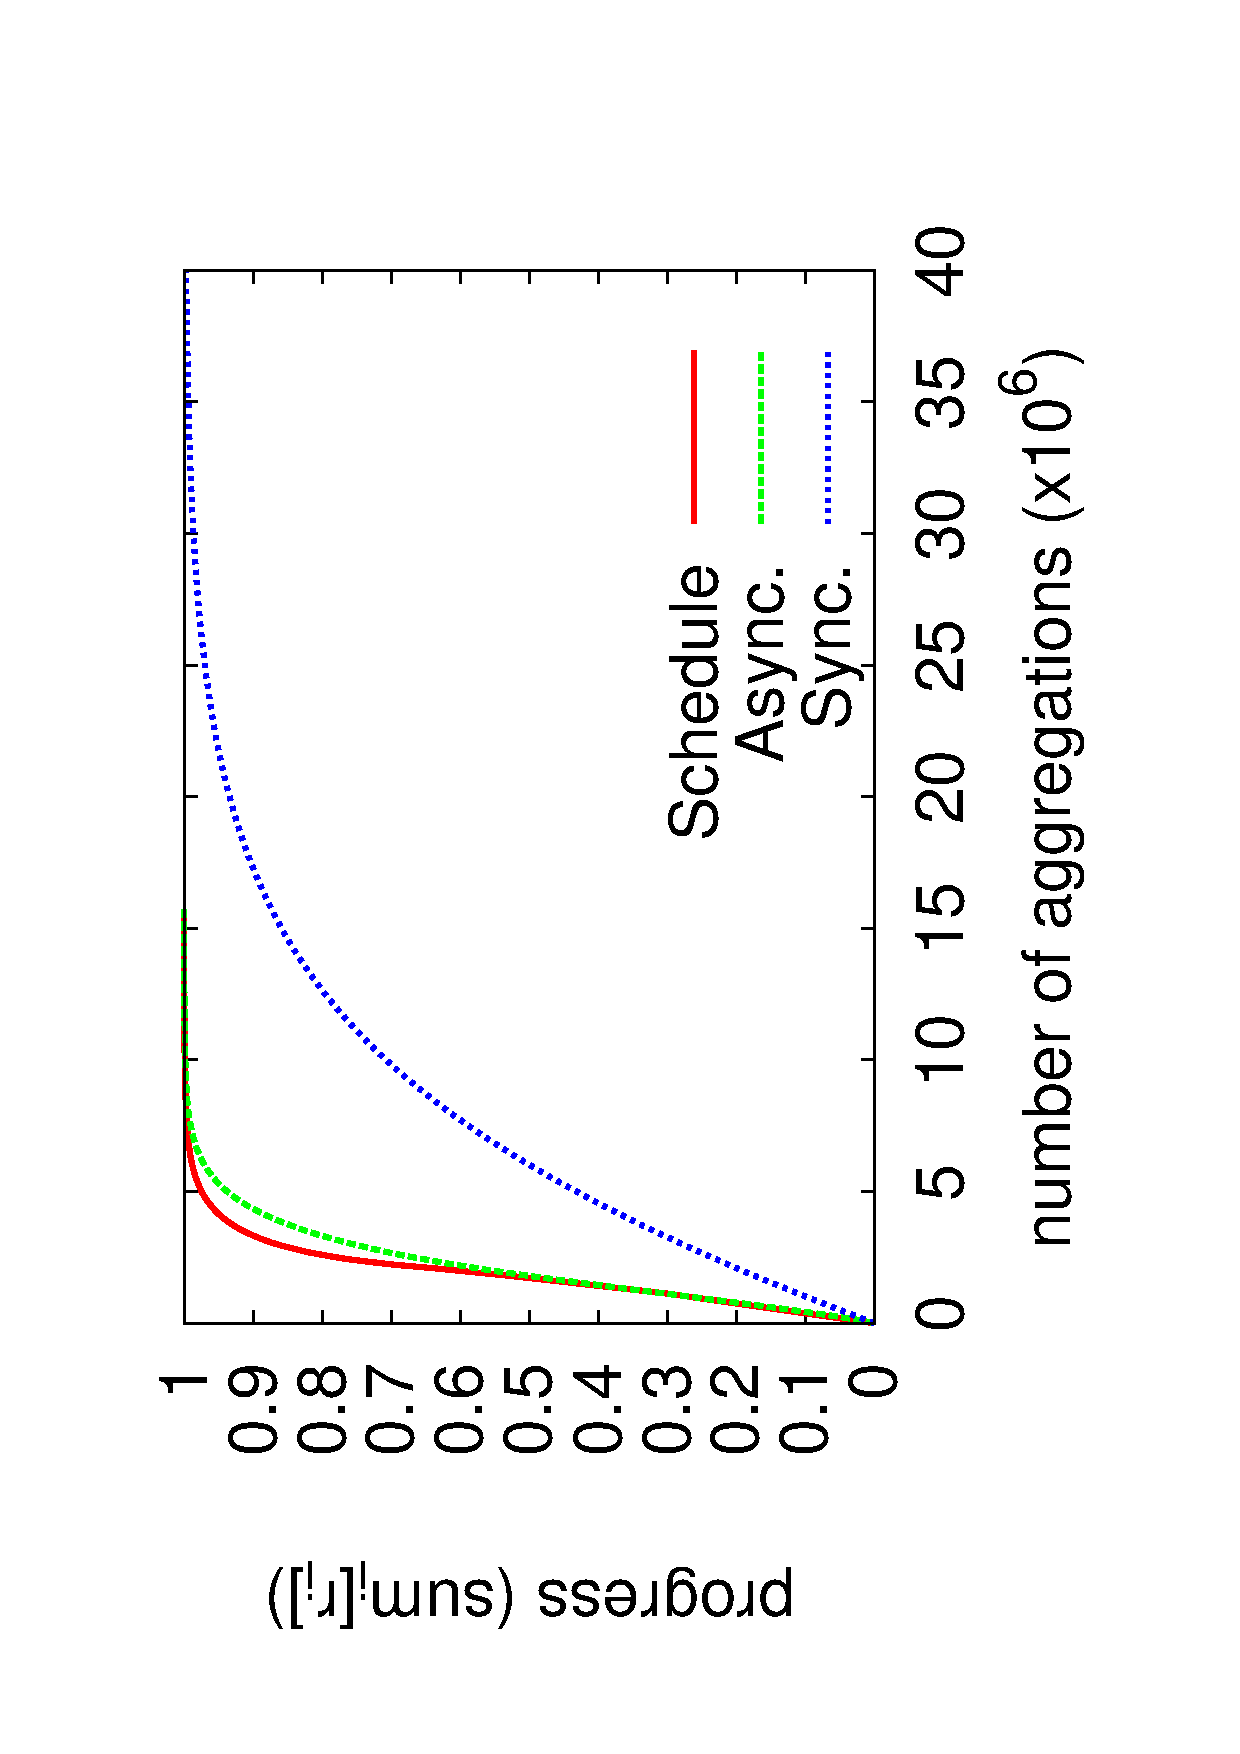
\includegraphics[width=1.3in, angle=-90]{fig/roadca_aggregate_progress}
    \label{fig:single-numagg:roadca}
    \vspace{-0.05in}}
    \hspace{-5mm}
    \subfloat[Livejournal]{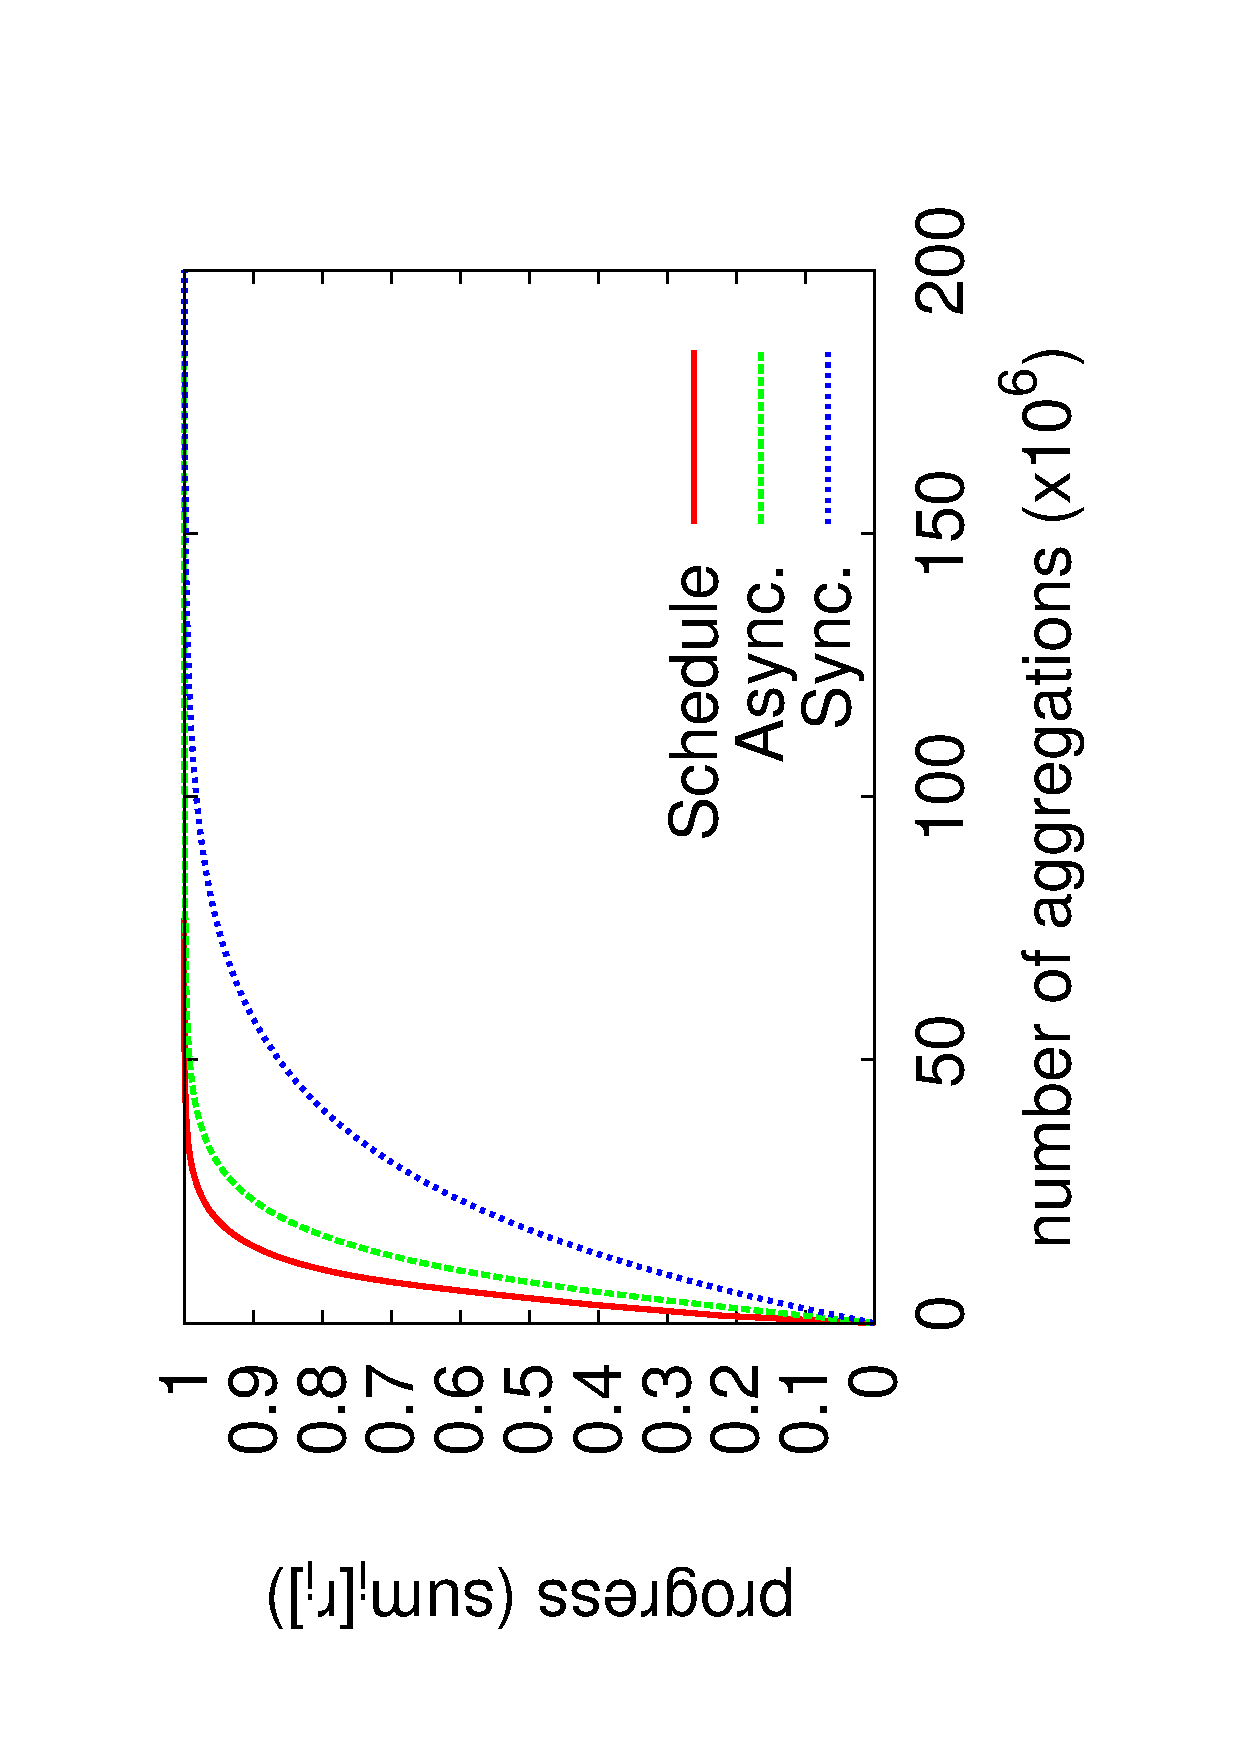
\includegraphics[width=1.3in, angle=-90]{fig/livejournal_aggregate_progress}
    \label{fig:single-numagg:livejournal}
    \vspace{-0.05in}}
    }
    \vspace{-0.1in}
	\caption{Effectiveness of aggregate operations to converging progress}
	\label{fig:single-numagg}
\vspace{-0.1in}
\end{figure}

The effectiveness of aggregate operations in asynchronous aggregation is an important advantage but tends to be underestimated. Synchronous aggregation requires to aggregate the information from previous iteration, while asynchronous aggregation accumulates the most up-to-date information. Thus, the aggregate operation is expected to be more effective. In this experiment, we evaluate the effectiveness of aggregations on accelerating the computation progress.

We run PageRank on two datasets, RoadCA and Livejournal, which result in the most speedup and the least speedup comparing to synchronous aggregation as shown in Table \ref{tab:wrokload}. We record the accumulated number of aggregate operations during the computation. In the accumulated version of PageRank (see Sec. \ref{sec:async:convert}), the summation of ranking scores $\sum_i{r_i}$ is approaching to 1 and will finally converge to 1. So we estimate the computation progress by evaluating $\sum_i{r_i}$ periodically. Fig. \ref{fig:single-numagg} shows the results. By using asynchronous aggregation, the converging progress is much faster than using synchronous execution. The scheduling of aggregate operations will further speedup the progress. The asynchronous aggregation with scheduling shows more effectiveness, so that each aggregate operation contributes more. It also shows more effectiveness on the RoadCA graph than on the Lievejournal graph. This is the reason why higher speedup is observed on the RoadCA graph.



%\subsection{Communication Cost}
%\label{sec:expr:communication}

%Asynchronous aggregation has the advantage of avoiding network congestion during synchronization phase.


% that's all folks
\end{document}


